% Options for packages loaded elsewhere
\PassOptionsToPackage{unicode}{hyperref}
\PassOptionsToPackage{hyphens}{url}
%
\documentclass[
]{book}
\usepackage{amsmath,amssymb}
\usepackage{iftex}
\ifPDFTeX
  \usepackage[T1]{fontenc}
  \usepackage[utf8]{inputenc}
  \usepackage{textcomp} % provide euro and other symbols
\else % if luatex or xetex
  \usepackage{unicode-math} % this also loads fontspec
  \defaultfontfeatures{Scale=MatchLowercase}
  \defaultfontfeatures[\rmfamily]{Ligatures=TeX,Scale=1}
\fi
\usepackage{lmodern}
\ifPDFTeX\else
  % xetex/luatex font selection
\fi
% Use upquote if available, for straight quotes in verbatim environments
\IfFileExists{upquote.sty}{\usepackage{upquote}}{}
\IfFileExists{microtype.sty}{% use microtype if available
  \usepackage[]{microtype}
  \UseMicrotypeSet[protrusion]{basicmath} % disable protrusion for tt fonts
}{}
\makeatletter
\@ifundefined{KOMAClassName}{% if non-KOMA class
  \IfFileExists{parskip.sty}{%
    \usepackage{parskip}
  }{% else
    \setlength{\parindent}{0pt}
    \setlength{\parskip}{6pt plus 2pt minus 1pt}}
}{% if KOMA class
  \KOMAoptions{parskip=half}}
\makeatother
\usepackage{xcolor}
\usepackage{longtable,booktabs,array}
\usepackage{calc} % for calculating minipage widths
% Correct order of tables after \paragraph or \subparagraph
\usepackage{etoolbox}
\makeatletter
\patchcmd\longtable{\par}{\if@noskipsec\mbox{}\fi\par}{}{}
\makeatother
% Allow footnotes in longtable head/foot
\IfFileExists{footnotehyper.sty}{\usepackage{footnotehyper}}{\usepackage{footnote}}
\makesavenoteenv{longtable}
\usepackage{graphicx}
\makeatletter
\def\maxwidth{\ifdim\Gin@nat@width>\linewidth\linewidth\else\Gin@nat@width\fi}
\def\maxheight{\ifdim\Gin@nat@height>\textheight\textheight\else\Gin@nat@height\fi}
\makeatother
% Scale images if necessary, so that they will not overflow the page
% margins by default, and it is still possible to overwrite the defaults
% using explicit options in \includegraphics[width, height, ...]{}
\setkeys{Gin}{width=\maxwidth,height=\maxheight,keepaspectratio}
% Set default figure placement to htbp
\makeatletter
\def\fps@figure{htbp}
\makeatother
\setlength{\emergencystretch}{3em} % prevent overfull lines
\providecommand{\tightlist}{%
  \setlength{\itemsep}{0pt}\setlength{\parskip}{0pt}}
\setcounter{secnumdepth}{5}
\usepackage{booktabs}
\ifLuaTeX
  \usepackage{selnolig}  % disable illegal ligatures
\fi
\usepackage[]{natbib}
\bibliographystyle{plainnat}
\usepackage{bookmark}
\IfFileExists{xurl.sty}{\usepackage{xurl}}{} % add URL line breaks if available
\urlstyle{same}
\hypersetup{
  pdftitle={XOXO Community Survey 2024},
  pdfauthor={Beth M. Duckles},
  hidelinks,
  pdfcreator={LaTeX via pandoc}}

\title{XOXO Community Survey 2024}
\author{Beth M. Duckles}
\date{2024-10-31}

\begin{document}
\maketitle

{
\setcounter{tocdepth}{1}
\tableofcontents
}
\chapter{XOXO Community Survey 2024}\label{xoxo-community-survey-2024}

\section{What This Is}\label{what-this-is}

This is a vibe check community survey of the \href{https://xoxofest.com/}{XOXO Fest Slack community}.

In early October 2024, Andy McMillan and Andy Baio (sometimes collectively referred to as ``the Andys'') who are the organizers of the festival and the Slack announced that because the festival ended, they would be closing down the XOXO Slack community that has been a mainstay of the community since the beginning of the festival.

In response to this announcement, some folks suggested we might want to do a survey to discuss next directions. These directions included: which platforms folks wanted, what their concerns were about the closure and what positive directions this shift might take.

We also wanted to give people a chance to share their feelings and emotions about the shift and to share their gratitude.

Beth Duckles put together this survey to solicit community feedback. We put it out on October 9th, 2024 and gave the existing Slack community about a week to respond. We received 154 responses.

Analysis was done by Beth Duckles and Rosa Quiñones, the report was written by Beth Duckles with editing and feedback from Benjamin Chait, stacy-marie ishmael, Matt Lee, Josh Millard, Rosa Quiñones, Nora Ryan, Pete Modica-Soloway and David Werthheimer.

\section{How We Did It}\label{how-we-did-it}

This report summarizes the findings of the survey responses and identifies key themes.

Our goal was to provide materials that would contribute to a community discussion, rather than an exhaustive categorization of every comment. By reflecting what we saw/read in the data, we're hoping to give more data to the conversation.

Beth and Rosa organized the comments for each question into themes as a way to share the information that came from the survey. In each theme, we share quotes in bullet points that describe what we saw relating to that theme.

This grouping of responses into themes was done very quickly. Our goal was for the community to have something fast rather than something perfect (and long-delayed). There may be themes you identify in the data we didn't highlight, or categorizations that you might have approached differently.

\section{The Data}\label{the-data}

There is a lot here, so we understand that you may need time to process all of it.

Listening to the many voices of other people involves letting their words be at the center, which means we highlight lots of quotes. You will sometimes see the same quote in multiple places.

In this kind of research \textbf{we don't edit what people write in their response to the survey}. This means that if there are typos in survey responses, those are reflected without editing here.

\section{Gift}\label{gift}

This survey and research are a gift freely offered to a community that has given us so so much.

Beth does work like this for communities as a research consultant and would be happy to talk to you about doing research for communities you're a part of. She was able to do this work because of some freedom in her schedule and is always looking for new clients. If you want to talk to her about research projects for hire or want to drop a few bucks her way, find her on the Slack at bduckles or her email: \href{mailto:beth@duckles.com}{\nolinkurl{beth@duckles.com}} or online at \href{https://bethduckles.com/}{Beth Duckles}.

\chapter{Executive Summary}\label{executive-summary}

The first section of the report can be seen as a discussion of the values, impact and gratitude for the XOXO Community

\textbf{\href{https://bduckles.github.io/XOXOReport_BD/community-values.html}{Chapter 3 - Community Values}}

\subsection{The Community}\label{the-community}

The values of the XOXO Community as expressed in the survey were the focus on: kindness and empathy, creativity, inclusivity, curiosity, emotional intelligence and community.

\textbf{\href{https://bduckles.github.io/XOXOReport_BD/appreciation-for-the-community.html}{Chapter 4 - Appreciation For the Community}}

When asked what people appreciated about the community:

\begin{itemize}
\tightlist
\item
  They remarked first and foremost on the \textbf{people} in the community and the the diversity of perspectives.
\item
  Folks talked about using the Slack as a \textbf{resource} or a place to ask questions, gain information, to learn new things, to read the news, and to find links.
\item
  They described the \textbf{shared values} in the community such as upholding a sense of kindness, a political alignment and the idea that one should act without creating harm.
\item
  People referred to the community as a place for \textbf{kind and empathetic humans} and they valued creating a safe place with privacy and openness.
\end{itemize}

\textbf{\href{https://bduckles.github.io/XOXOReport_BD/impact.html}{Chapter 5 - Impact}}

When asked about the impact of the XOXO community on their lives

\begin{itemize}
\tightlist
\item
  folks discussed with the \textbf{quality of the community} and how they had brought much of that way of thinking into other aspects of their lives.
\item
  From \textbf{meeting good people}, finding friendships, feeling at home, to being welcomed the XOXO community was a space that folks pointed to to show what community can be.
\item
  Folks talked about it feeling like the \textbf{``old internet''} or ``old twitter''.
\item
  Respondents spoke about the \textbf{resources} they gained in the community, the \textbf{personal growth} they experienced, the richness of the conversations they had.
\item
  Folks talked about specific channels that had been impactful for them. During hard times, specifically during Covid, the Slack has been a ``lifeline'' and supported folks in their mental health and well being.
\end{itemize}

\subsection{What Happens Next}\label{what-happens-next}

The second part of the report can be seen as a discussion of what happens next:

\textbf{\href{https://bduckles.github.io/XOXOReport_BD/concerns.html}{Chapter 6 - Concerns}}

\begin{itemize}
\tightlist
\item
  Many folks feared the \textbf{loss of the community}, of the connections, of the resources and special XOXO spirit.\\
\item
  Responses reflected a fear that the community will \textbf{splinter, fracture or fragment} going forward.
\item
  They described \textbf{concerns} about new platforms, leadership and specific community needs.
\end{itemize}

\textbf{\href{https://bduckles.github.io/XOXOReport_BD/platforms.html}{Chapter 7 - Platforms}}

The top three platform contenders were Discord, Slack and Discourse. Functionality on both computers and mobile is important for this community.

\textbf{\href{https://bduckles.github.io/XOXOReport_BD/platform-opportunities.html}{Chapter 8 - Platform Opportunities}}

\begin{itemize}
\tightlist
\item
  Respondents said they could see some \textbf{positive changes} that a platform change could have for the community: it could signal an expansion, an evolution or a refresh of the community.
\item
  Folks talked about being \textbf{intentional} about next steps and some of the opportunities that exist for decentralization.
\item
  There was a sense that there could be changes in organization, moderation and making sure the \textbf{community was sustainable.}
\item
  Others talked about the desire for \textbf{new ideas, people, resources and events.}
\item
  Some also spoke of particular features and benefits that might come from changes by using \textbf{Discord} in particular.
\end{itemize}

\textbf{\href{https://bduckles.github.io/XOXOReport_BD/platform-concerns.html}{Chapter 9 - Platform Concerns}}

\begin{itemize}
\tightlist
\item
  Concerns included worrying that folks would disperse, we'd lose the network, the new platform would be unfamiliar and there'd be a loss of resources.
\item
  Some focused on challenges with \textbf{leadership structures}, moderation, costs and loss of the XOXO spirit.
\item
  Some discussed \textbf{functions in platforms} that could be possible with changes as well as specific comments about various platforms.
\end{itemize}

\textbf{\href{https://bduckles.github.io/XOXOReport_BD/name.html}{Chapter 10 - Name}}

The top contenders for names are:

\begin{itemize}
\tightlist
\item
  And, And/\&\& (8)
\item
  Enthusiasm Collective (8)
\item
  Good Internet (7)
\item
  Lowered Expectations/LoX/LOX/LowEx (5)
\item
  YNYN (2)
\item
  TKTK (2)
\item
  Good Together (2)
\end{itemize}

\subsection{Thank you}\label{thank-you}

The final chapter is a thank you to the Andys.

\textbf{\href{https://bduckles.github.io/XOXOReport_BD/thank-you-to-the-andys.html}{Chapter 11 - Thank You}}

Dear Andys,

You're the best, we think the world of you. You made a community, one that was kind and that helped us remember the good internet. We saw how hard you worked. You changed lives and you should be proud of what you've done. We are so grateful and we the community will take it from here. Thank you.

Love, the XOXO community

\textbf{\href{https://bduckles.github.io/XOXOReport_BD/appendix---survey-questions.html}{Appendix - Survey Questions}}

\chapter{Community Values}\label{community-values}

The question we asked was: ``If you were to briefly summarize the core values of the XOXO Slack Community as it exists now, what would they be?

Many folks responded with a string of words separated by commas, so I pulled those apart, counted them and collapsed where appropriate (e.g.~creative, creativity and creations became creativity). Others wrote a phrase or a sentence and those are interspersed in the discussion where they added to the themes.

The most popular words folks used were: (approximate number in parentheses):

\begin{itemize}
\tightlist
\item
  Empathy (27)
\item
  Kindness (26)
\item
  Creative (25)
\item
  Openness (14)
\item
  Community (15)
\item
  Curiosity (13)
\item
  Inclusivity (12)
\item
  Thoughtful (11)
\item
  Support (9)
\item
  Compassionate (9)
\item
  Fun (7)
\item
  Caring (6)
\item
  Respect (6)
\item
  Enthusiastic (5)
\item
  Helpful (5)
\item
  Generosity (4)
\item
  Friendly (3)
\item
  Sharing (3)
\end{itemize}

I grouped the words together in themes that I came up with based on what folks wrote/said. I added quotes to match the groupings. All groupings are open to discussion/interpretation and clearly there is a lot of overlap.

\section{Kindness and Empathy}\label{kindness-and-empathy}

The value of kindness and empathy took many forms: compassionate, helping, a caring community, connecting and nurturing, gentle, kind, wholesome-ness, earnest, empathy, integrity.

Quotes that discuss kindness:

\begin{itemize}
\tightlist
\item
  Supportive \& honest, and a kind place to be on the internet.
\item
  Empathy. A safe space to act like a social network without worrying about the bad parts of the internet.
\item
  Compassionate, empathetic, engaged community caring for each other's creative pursuits to become more whole humans.
\item
  Creativity and empathy driven kindness
\item
  Empathy and kindness centered willingness to be hyped up about almost anything
\item
  caring and helpful
\item
  Empathy and creativity. We are people who have been brought together by caring about making things thoughtfully in community with others, and that if you are emotionally vulnerable about the difficulties of that journey it will be paid back with kindness and a sense of unity
\item
  Kindness, patience, and passion. Also, showing or trying for best practices for lots of things --- inclusion, managing and sharing emotions appropriately (the \#bad-attitude channel), the reactji people added
\end{itemize}

\section{Creativity}\label{creativity}

Creative was often used to describe the community, and it seemed to also encompass the idea of artistry and a sense of fun. Folks used words like: enthusiastic, humor, entertaining, exciting, making weird stuff for fun, playful, sharing fun things, sharing neat projects and weirdness.

Some quotes around this theme:

\begin{itemize}
\tightlist
\item
  Give creative, smart, good-hearted people a safe way to express themselves, connect with others, learn to share themselves with the world, and live fulfilling sustainable creative lives.
\item
  A welcoming community for the best weirdos the internet has to offer
\item
  A community of people who build good internet-related things (loosely defined). People who are humane and humorous. People who want to share things that they find joyful.
\item
  Creative, curious, KIND people. Safe space to explore ideas and thoughts about life and creative work!
\item
  take joy in the things around you; celebrate things that are cool; celebrate each other; assume good faith; it's OK to not be OK; fuck {[}elon / trump / DHH / tech-or-politics-adjacent weirdo of the week{]}
\item
  Making things. Remaining independent.
\item
  Knowledge \& awareness; earnest love of the weird and silly; thoughtful and playful uses of technology (esp.~The Internet); mutual respect and care
\end{itemize}

\section{Inclusivity}\label{inclusivity}

Words people used to describe the community around the idea that it's open and inclusive. They also used words like: respect, friendly, helpful, encouragement, inviting, welcoming, inclusiveness.

While the words inclusivity and openness were used, some also described the community being closed as part of this inclusivity. Some called it safe, a safe haven or safe space for expressing thoughts. Additionally others talked about it being also a place where there was privacy and also confidential-ish.

Quotes around inclusivity and openness:

\begin{itemize}
\tightlist
\item
  Openness, curiosity, fun, belief that the internet can be a wonderful, creative place.
\item
  Safe spaces, where people feel comfortable to be their true authentic selves. Inclusivity, where everyone is welcomed, seen and heard. Encouragement and support in all aspects of life, from local classifieds-type of sharing, to deeper and more personal concerns.
\item
  having a safe community that supports each other
\end{itemize}

\section{Curiosity}\label{curiosity}

Words people used to describe the value of curiosity include: insightful, interest, knowledge sharing, news sharing, resource sharing, resourcefulness, smart, thoughtful discussion, Curiosity, Interesting, learning, understanding, exploration. As we'll see later, many folks said that the community was smart and that they appreciated the level of intelligence in discourse.

Quotes around curiosity and intelligence:

\begin{itemize}
\tightlist
\item
  Super bright people who are really nice and very tech savvy
\item
  Smart creative folks sharing and helping each other.
\item
  the confluence of curiosity, expertise and community
\item
  low-stakes learning community
\item
  Thoughtfully sharing highlights of the internet, commentary, empathy, joy, and advice
\item
  Interesting news, events, and discussions that I don't find anywhere else
\end{itemize}

\section{Emotional Intelligence and Integrity}\label{emotional-intelligence-and-integrity}

Folks seemed to convey a value in the community around emotional intelligence, though it wasn't always named this. Some example phrases: acknowledgment of feelings, earnest good vibes, listening (before fixing), getting consent, space for feeling feelings and witnessing others, meta communication, communication as a skill and keeping the bad vibes in their own channels.

Similar sentiments could be found in a sense of integrity in the community such as words like thoughtful, respect, respectful, civility, honesty, humanity, principled, respectful, and sincerity.

Quotes:

\begin{itemize}
\tightlist
\item
  Everyone is valuable and deserves to be treated with respect.\\
\item
  Acceptance of others and their ideas. Breadth and diversity of userbase.
\item
  Mutual support/big sense of community , interest in others ideas, joy of sharing and supporting, doing our best to make sure everyone is thoughtfully heard and included
\end{itemize}

\section{Community}\label{community}

Quite a few people used words that related to the idea of community such as: support, sharing, acceptance, generosity, mutual support, supportive, camaraderie, mutual aid, togetherness, care for each other, cooperation, equity, giving voice to the marginalized, giving others the benefit of the doubt, lifting each other up, mutual respect, togetherness, authenticity, tolerance, trust, utopianism and validation.

Quotes on community:

\begin{itemize}
\tightlist
\item
  thoughtful community based on lifting up and informing each other
\item
  Inclusive community
\item
  Unique set of people with a lot of things in common that supports each other and shares good stuff
\end{itemize}

\section{Overall Values Statements}\label{overall-values-statements}

Some folks shared phrases that seemed to be more general and to encompass several of the values above.

\begin{itemize}
\tightlist
\item
  Collective hive-mind of support, creativity, appreciation for art with a set of overlapping societal principles that steer healthy moderation and a general openness to new dialogue or change.
\item
  Be the internet you want to see in the world
\item
  a commitment to the good parts of the web
\item
  A like-minded community conscientious of etiquette, while encouraging curiosity and discovery without competing for popularity or ostracizing members.
\end{itemize}

\section{Additional Quotes/Comments}\label{additional-quotescomments}

\begin{itemize}
\tightlist
\item
  I don't know that there are strong core values that come from the slack itself. I think it is in many ways a reflection of the event rather than it's own community with a sense of identity
\item
  To me, it was more than just a companion piece to the physical festival. I attended a few times, regretted not going the first year, and missed out on securing a spot in the last year. It was the crossroads of art, culture, and techology from a group of what felt like inclusionary, progressive and small ``l'' liberal people that agreed to operate under a code of conduct that emphasized politeness and kindness in a time when those things are not the norm (online or in public).
\item
  Progressivism, humanism, and a love for all things indie
\end{itemize}

\chapter{Appreciation For the Community}\label{appreciation-for-the-community}

The question we'll discuss in this section was ``What do you appreciate about the XOXO Slack community?'' Unsurprisingly, this mirrored much of what was discussed in the values section, but with deeper explanation.

This section is split into three subsections: folks shared appreciation for the people, the resources in the community and the shared values.

\section{The People}\label{the-people}

By far, the overwhelming response to this question of what folks appreciate about the Slack is the other people in the Slack.

\begin{itemize}
\tightlist
\item
  I feel like I found my people here.
\item
  The caliber of people and the fact that it's about as safe of a space as I could imagine existing online. It might actually be the safest space online.
\item
  I appreciate the opportunity to connect with all the wonderful people in the community. This group of intelligent, connected and, attentive people have enriched my existence in many ways, including just talking about important or interesting things in a relatively safe environment.
\item
  so many incredible people, so willing to help each other
\item
  The people, the various emoji that say a thousand words, the different channels for different topics, the thread-first approach to communicating, the organisation of everything thanks to folks like the moderators, and even the very active members I recognise!
\item
  everyone is so awesome and kind
\item
  the people, the thoughtful responses
\item
  Local subject matter experts, friendly people, good discussion
\item
  People who are like me, openly sharing who they are, sharing advice, support, empathy and making every experience shared and a little less hard
\item
  The lovely humans that make up the community and how they interact with each other
\item
  It's an amazing place of creative people who are generous, kind, and a lot of fun. Also Andy Baio finds the best links.
\item
  The ability to assume truthfulness or good faith in the things that are shared, and the ability to be possibly wrong, possibly clumsy, possibly human
\item
  The way everyone embodies the value above and leads through their actions
\item
  the people, the content, the kindness, the attitudes, and the opportunity for closer conversations with lovely people
\item
  The XOXO Slack community is helping and giving. People care. People are enthusiasic about things! People are really smart and interesting!
\item
  People's willingness to be vulnerable and to hold space for others to be vulnerable
\item
  All of those core values! And the sheer interestingness of the members of the community
\end{itemize}

\subsection{Diversity of Perspectives}\label{diversity-of-perspectives}

One of the attributes of the people that folks commented on was how many diverse perspectives they felt could be found in the slack.

\begin{itemize}
\tightlist
\item
  The people who are on it, come from a lot of different perspectives and backgrounds and that makes it more interesting
\item
  The variety of backgrounds and perspectives of participants
\item
  Diversity of perspectives, freely given knowledge, empathy and compassion for experiences, range of interests, learning and growing together
\item
  Such a breadth of experience and diverse skills in the members!
\item
  That it's far more of a diverse community --~along almost any axis, other than perhaps political leanings --~than I would ever have access to in my day to day life.
\item
  diversity, empathy, endless curiosity
\end{itemize}

\subsection{Portland}\label{portland}

Folks in Portland in particular talked about how useful the slack was to find things in their community.

\begin{itemize}
\tightlist
\item
  I'm a lurker, more than a poster. The \#portland slack has been incredibly valuable as a local. I've attended events, visited restaurants, learned about civic activities, and donated to causes I learned about via Slack.
\item
  For Portland especially, xoxo is a wonderful resource of news, vendors, events.
\item
  Its relative privacy and safety, most of the cool new things I've learned about in Portland and on the Internet were via this Slack.
\item
  It's been a really good resource for things going on in Portland Oregon! Otherwise it's just nice to see what people are up to or reading.
\item
  feels like the small room of good internet circa 2010-2015 and/or like Twitter before it got bad. Secondly, as a new native to Portland I really appreciate participating in a community of like-minded local creators
\end{itemize}

\section{Resources}\label{resources}

\subsection{Asking for Information}\label{asking-for-information}

Respondents discussed using the Slack to share knowledge, ask for help and to learn from one another. They described people being generous and helpful when they did so.

\begin{itemize}
\tightlist
\item
  I love having a place to keep up to date with links and stories shared in channels plus a place to connect and ask questions on a variety of topics.
\item
  When I have a question about damn near anything (resource, fact, local stuff, whatever) someone knows the answer and is likely to be similar enough in mindset to me that I can trust it. And, the goofy shit I like to share always seems to find an appreciative crowd
\item
  Breadth of channels. I can ask/answer Maker or home-improvement questions, keep up to date on tech/politics, and see folks being happy about stuff they made or found.
\item
  People's openness to help, share knowledge, and generally be excepting
\item
  When I have a question about damn near anything (resource, fact, local stuff, whatever) someone knows the answer and is likely to be similar enough in mindset to me that I can trust it. And, the goofy shit I like to share always seems to find an appreciative crowd
\item
  Being able to ask all the dumb questions about anything and everything, and having really smart, capable people reply with their wisdom and resources
\item
  Ability to ask kind individuals both hard and easy questions across a variety of topics
\item
  People who are like me, openly sharing who they are, sharing advice, support, empathy and making every experience shared and a little less hard
\item
  Diversity of perspectives, freely given knowledge, empathy and compassion for experiences, range of interests, learning and growing together
\item
  Feedback and support
\item
  Quality information
\item
  I appreciate the broad range of skills and expertise. I also love that we all are passionate about something and we're open to hearing about other's passions.
\item
  the ability to drop in and engage, the willingness of the community to provide support (responses, engagement, advice, etc.) and the depth and breadth of knowledge across all its members
\item
  I like that I have a place to hear about the things I'd hear about on social media (news, tech news, neat creative projects, dumb jokes) without the context collapse of social media, and in a moderated and kind environment. As a curated microcosm of the internet at large, I can dip my toe in and feel rewarded without getting hit with the anxiety and overwhelm - and the smaller scale means I've made some lasting friendships and connections because I'm able to show up more fully than I would if I was more afraid.
\item
  private identity channels; knowing that i can ask basic questions and people love info-dumping with no judgement
\item
  It's a large group of smart, successful, creative, people who as a whole, is good-internet. I've made friends and professional connections here and my favorite by-product is the community's ability to help me gather information on almost anything, which also spoils me because I'm not confident in my abilities to find reliable information through traditional web searches.
\item
  SO much. It's a place where I learn about and discuss current events and art with folks I like and admire. Also, frankly, it'a a place I can lurk! I expreience severe rejection sensitivity in online spaces, so the fact that I can pop a little emoji next to a post to show sympathy, curiosity, etc is really nice for me. I also experience the moderation as very present, compassionate, and firm, which REALLY makes a difference in the space.
\end{itemize}

\subsection{Learning}\label{learning}

Folks also discussed how important it was to learn from others in the slack and how much they had learned over time. People talked about how smart other folks in the Slack are and how intelligent the conversations were in the channels. They also described the space as being curated and having a variety of things they wouldn't otherwise see/hear about.

\begin{itemize}
\tightlist
\item
  I learn SO much. There's so many smart voices.
\item
  The smart creative, mostly likeminded folks.
\item
  Local subject matter experts, friendly people, good discussion
\item
  Honestly, the ``closed'' nature of the community worked for me for professional reasons. But I also loved the diversity of topics and how it let me get to know different people from the general community.
\item
  Being able to ask all the dumb questions about anything and everything, and having really smart, capable people reply with their wisdom and resources
\item
  From the delightful shared experience of the Animal Crossing channel in early Covid, to the freewheeling discussion of politics, to the creative problem solving and solidarity of many other channels, questions, learning and growth are supported and so are the personal connections we've forged at the festival and in this digital space.
\item
  empathy, wisdom of the crowd, discovery
\item
  Diversity of perspectives, freely given knowledge, empathy and compassion for experiences, range of interests, learning and growing together
\item
  knowledge base
\item
  Curious, smart, politically progressive
\item
  In depth and well meaning discussions on difficult topics - seeing people's various opinions and considerations help me form my own
\item
  A large amount of very smart people all feeling like it's a safe place to express their thoughts
\item
  It's a large group of smart, successful, creative, people who as a whole, is good-internet. I've made friends and professional connections here and my favorite by-product is the community's ability to help me gather information on almost anything, which also spoils me because I'm not confident in my abilities to find reliable information through traditional web searches.
\end{itemize}

\subsection{News}\label{news}

Folks also described the slack as the place that they used to find the news, and that they relied on each other to have compelling and interesting conversations about topics that were on the front page of the newspapers.

\begin{itemize}
\tightlist
\item
  a way to get news, to get fresh and useful perspectives on news (politics and tech, mostly)
\item
  Great source for news \& interesting projects from all around the internet, fantastic discussions with smart people who are experts on various topics
\item
  Resources in news/likeminded spirit
\item
  Discussions on the XOXO Slack are always my first choice for any online interaction, it's replaced all news sites
\item
  Excellent moderation, ability to check in for local Portland events plus national events (like politics and C19). My first go-to community for EVERYTHING, including classifieds.
\item
  Very up to date news, an active community, lots of channels dedicated to very specific topics
\item
  It's a place where I can stay abreast on the difficult topics of the modern digital world and remain connected to other digital artists without the terrible emotional pain that comes along with using social media like Twitter
\item
  Surfaces good posts and news (replaced social media). People there make me feel seen. We don't ramble, we share and support.
\item
  I don't like to consume news because of its ill effect on my mental health, and this Slack helps me stay engaged with issues I care about. I appreciate hearing the perspectives of this community.
\end{itemize}

\subsection{Cool Stuff People Share}\label{cool-stuff-people-share}

People described the benefit of being in a space where folks share cool stuff and they get to have curated content that they like.

\begin{itemize}
\tightlist
\item
  Being able to stay in touch with friends made at XOXO. Seeing and hearing about all the cool stuff people make and share, whether from within the community or elsewhere. Recommendations on local and online businesses for specific needs.
\item
  Great source for news \& interesting projects from all around the internet, fantastic discussions with smart people who are experts on various topics
\item
  Curated content, exclusive access, there are experts in everything
\item
  Fellow nerds and weirdos who read the internet so I don't have to. Also I like that sharing is encouraged. I'm not someone with any real online presence so it's nice having that space. Also, being able to have people productively disagree, though there have been a few instance of that being tested in the politics channel, the way it was handled by the Andy's was I think very good.
\item
  empathy, wisdom of the crowd, discovery
\end{itemize}

\subsection{Alternative to Media}\label{alternative-to-media}

Some folks talked about the community as a place where they could have a discussion that wasn't as broken as some of the media we have now.

\begin{itemize}
\tightlist
\item
  It's a group that cares about and wants the best from the Internet, but without the blind techno-Utopianism of mainstream tech culture.
\item
  I like that I have a place to hear about the things I'd hear about on social media (news, tech news, neat creative projects, dumb jokes) without the context collapse of social media, and in a moderated and kind environment. As a curated microcosm of the internet at large, I can dip my toe in and feel rewarded without getting hit with the anxiety and overwhelm - and the smaller scale means I've made some lasting friendships and connections because I'm able to show up more fully than I would if I was more afraid.
\item
  It's a place where I can stay abreast on the difficult topics of the modern digital world and remain connected to other digital artists without the terrible emotional pain that comes along with using social media like Twitter
\item
  A digital shelter from a capitalistic web
\item
  It helps keep me centered in a greedy, competitive world.
\item
  nice place for nerds to nerd out
\end{itemize}

\section{Shared Values}\label{shared-values}

Many folks talked about how they shared values with others in the community, including the upholding of the code of conduct, the sense of political alignment and a common belief in the idea that folks should be acting in ways that are not harmful.

\begin{itemize}
\tightlist
\item
  it's a community with a shared \emph{ethos} rather than shared subject matter, large enough to have lots of casual relationships/interactions but not the entire goddamn internet
\item
  It's the only social network that feels truly connected and wholesome. I use it to connect with a community of people that share my values, and know that the people sharing information care about the quality of their information, and will always act in the best interest of the community and each other. And if anybody acts in harmful ways, they will learn from their mistakes and act differently (or be removed from the community)
\item
  General political/social alignment, joyfulness, creativity, persistence of identity
\item
  A group with diverse backgrounds and experiences but shared values
\item
  Varied perspectives, but somehow lots of people with the same morals as you. Easy to make friends.
\item
  People who are like me, openly sharing who they are, sharing advice, support, empathy and making every experience shared and a little less hard
\item
  it's a collection of nice people who do interesting things, the whole community is invested in upholding the existing CoC/culture, the word ``building'' comes to mind (community/each other up/cool stuff/process/etc.)
\item
  Nearly everyone visible on Slack* appears committed to the core values of the Slack, providing a safe space for others, enforcing norms to that end, and politely accepting correction from others. There is a general understanding that not all behavior or speech can be welcome and still offer the safety needed to help people be and grow true to themselves. (*Behavior outside of this range may be happening and is not visible due to vigilant moderator efforts.)
\item
  It's the only social network that feels truly connected and wholesome. I use it to connect with a community of people that share my values, and know that the people sharing information care about the quality of their information, and will always act in the best interest of the community and each other. And if anybody acts in harmful ways, they will learn from their mistakes and act differently (or be removed from the community)
\item
  Learning from the breadth of knowledge and experience of my Slack pals in a place where we tacitly acknowledging shared beliefs that I can't assume are shared everywhere (caring for other people, respecting other people's experiences and privacy)
\end{itemize}

\subsection{Kindness}\label{kindness}

Many, many people in the survey described the community as kind. Some examples:

\begin{itemize}
\tightlist
\item
  I have a group of kind, caring humans who give a shit.
\item
  Open minded people, kindness and empathy centered, a bastion of covid-awareness.
\item
  I appreciate how people are supportive and share their thoughts
\item
  Positivity, curiosity.
\item
  People who are like me, openly sharing who they are, sharing advice, support, empathy and making every experience shared and a little less hard
\item
  The kindness and enthusiasm
\item
  Same thing! All the creative, kind people. The commitment to inclusivity and authenticity
\item
  everyone is so awesome and kind
\item
  The kindness, the knowledge, the generosity of spirit of everyone involved.
\item
  everyone is so nice and we assume best intentions! also each account is one real person who has presumably interacted with the other people here IRL at least once, as part of a larger network (which lends some accountability/responsibility)
\item
  People are nice to each other. There are regular characters. The usual Slack conveniences that make it possible for people to not repeat themselves and to let me ignore US politics if I want to.
\item
  the small acts of kindness or indications of support people offer each other; emoji indications or threaded replies have genuinely lifted my spirits
\end{itemize}

\subsection{Safety}\label{safety}

One of those shared values seemed to be safety. People consistently referred to the slack as a safe space, or a place were they felt they could be themselves. They also commented that this made the space trustworthy and easy to be in.

\begin{itemize}
\tightlist
\item
  people assume good intent and read with compassion and reply with civility; it's a safe space for people with marginalized identities, people are funny and kind and creative and there's very little `rock star' attitude (even from people who are literally rock stars)
\item
  The safety and established trust.
\item
  The caliber of people and the fact that it's about as safe of a space as I could imagine existing online. It might actually be the safest space online.
\item
  It seems like both a safe place for optimism and constructive criticism.
\item
  A safe place for me to land for professional and personal needs
\item
  I love having a place full of people I respect and admire, where I nonetheless feel safe being honest and vulnerable.
\item
  It is consistently the kindest space I'm a part of. It's also the largest space I'm a part of that feels private and provides safety in its privacy.
\item
  Such a thoughtful space! I do not know how much moderation it requires, but from the outside it is a smoothly functioning space full of independent-minded folks, which is no small thing! I feel safe and cared about, even by relative strangers.
\end{itemize}

People also described this as a place with people they could trust

\begin{itemize}
\tightlist
\item
  My views align with those around me, and I enjoy chatting with people who share common ground. Since we all respect the code of conduct, there's less negative behavior, making interactions smoother. I value learning from the random, niche interests everyone brings, as someone always has expertise in something I'm curious about. These diverse perspectives help me expand my understanding and knowledge.
\item
  The broad spectrum of experiences and knowledge so that I can find out about a lot of different topics, from people who I feel like I can trust because they've been vetted.
\end{itemize}

\subsection{Privacy}\label{privacy}

Some folks linked safety with the privacy of the space.

\begin{itemize}
\tightlist
\item
  It is consistently the kindest space I'm a part of. It's also the largest space I'm a part of that feels private and provides safety in its privacy.
\item
  Honestly, the ``closed'' nature of the community worked for me for professional reasons. But I also loved the diversity of topics and how it let me get to know different people from the general community.
\item
  The wide world will never see it so I can really be myself
\end{itemize}

\subsection{Community}\label{community-1}

People discussed community as something that they felt a part of, that was important to them and that they shared with others.

\begin{itemize}
\tightlist
\item
  It's a very welcoming community, there's a shared sense of how hard it is to make things and an appreciation of what people do
\item
  It gives me a hometown, which I haven't had in ages and ages
\item
  I like how people don't jump to knives at the first opportunity, and appreciated that an Andy would step in and lay down the kindness law, gently then firmly, if needed, while not putting down one side or the other. I also like how people are able to browse and find others who have similar interests by looking at the channel list. I like that there are private spaces, as well. I also appreciate the `benevolent dictators' both the structure but also that our dictators are kind, patient, and passionate.
\item
  The ease of re-engaging after varying levels of activity, but also a core group of active members. This is the only only community I've belonged to where I feel most comfortable expressing opinions and not competing for popularity. In other social networks, I'm often forced to create separate identities for friends/family, private, and professional audiences.
\item
  the ability to drop in and engage, the willingness of the community to provide support (responses, engagement, advice, etc.) and the depth and breadth of knowledge across all its members
\item
  it's a collection of nice people who do interesting things, the whole community is invested in upholding the existing CoC/culture, the word ``building'' comes to mind (community/each other up/cool stuff/process/etc.)
\item
  it sits perfectly at the intersection of art, technology, nerdery, and social good. there are plenty of communities that bridge two of those things but I haven't found another that covers off on all of them like XOXO does.
\item
  The ability to communicate with others across multiple points of interest and the opportunities for mutual aid through ideas, concepts, and real world help.
\item
  Connection. This community has gotten me through some really hard times and while I may not know many of the folks here in person, I consider many of them friends.
\item
  \#portland and \#classifieds for local connection, \#good-internet / \#politics-and-news / \#tech-culture to keep up with relevant news and events
\item
  Ability to vent and then find distractions and cool things and inspiration
\item
  So many things. It's a place to go with wild ideas, or burning questions, or amusing anecdotes. It is a place to be supported and to give support.
\end{itemize}

\subsection{Openness}\label{openness}

People also described the community as open:

\begin{itemize}
\tightlist
\item
  People's openness to help, share knowledge, and generally be excepting
\item
  Open minded people, kindness and empathy centered, a bastion of covid-awareness.
\item
  Openness, creativity, sharing and support
\item
  that it's open, helpful, welcoming, entertaining
\end{itemize}

\chapter{Impact}\label{impact}

We asked the community: What would you like to share publicly about how the XOXO Slack has impacted your life?

\section{Quality of the Community}\label{quality-of-the-community}

Responses talked a lot about the quality of the community and how the community felt like an example to them of what good community and good internet could look like.

\begin{itemize}
\tightlist
\item
  XOXO Slack is one of the only online spaces where I feel like I'm connecting with an actual community of people willing to give me consideration as a person, where I can try new things, make mistakes, and trust that I'll receive both well-meaning feedback and forgiveness. We can chat and share casually about a wide range of topics without so much concern about a hypothetical future entity using what we say against us disingenuously. I can strive to be a good person, and not just self-censor to where I look like one.''
\item
  This community has changed my life. I've made lasting friendships and received career altering advice and assistance from the generosity and intelligence of the people assembled.
\item
  XOXO slack is hugely important to me as a source of community. Also (and far less importantly) I get a lot of cool links from the slack that I use to make it seem like I'm cooler in other communities
\item
  Xoxo slack provided community during the darkest time of the pandemic (and beyond) . I often feel isolated from creative communities which can be cliquish. Xoxo slack is the best type of inclusive community: bringing people together to learn and grow as responsible creative beings on this planet.
\item
  This community has been the closest to feeling like ``my people'' of anything I have ever experienced. People here have been consistently welcoming and friendly. I learn about things I otherwise would have missed on an almost-daily basis. I feel honored to have this kind of access to so many amazing folks. XOXO and this community have encouraged me to be less shy about sharing things I do and make.
\item
  I have always struggled to find a home on the internet. It's hard to join an existing community, and it's also hard to create one yourself. The XOXO slack always felt like such a welcoming place to just be. I really appreciate what it has been, and will miss it dearly -- but I look forward to whatever is next.
\item
  The XOXO slack is the first place on the internet where I felt at home.
\item
  I have always struggled to find a home on the internet. It's hard to join an existing community, and it's also hard to create one yourself. The XOXO slack always felt like such a welcoming place to just be. I really appreciate what it has been, and will miss it dearly -- but I look forward to whatever is next.
\end{itemize}

\subsection{An Example of Community}\label{an-example-of-community}

Folks referred to the community as something they point to as a good example of what community can be.

\begin{itemize}
\tightlist
\item
  Hard to define because it's been an accumulation of small things that have contributed to my whole identity. I'm not just my job, or my work, or my movements --- I'm also part of this community, this culture. The examples you all set have informed how I try to act and be, both online and offline. And of course the Andys' example of collaboration and leadership will always be a part of everything I do with others.
  It's taught me how to be more inclusive
\item
  this Slack has shaped my thinking about communities and how they work, as well as being an incredible support and resource during a very intense period of my life and in the world. it's one of the only places where I still seek out news and politics, partially because of the ethos of the space. oh! and it's where I found one of my closest co-workers for a couple of years, who is still a very good friend. during a period when so much of the internet became completely unbearable, the xoxo slack remained a constant reminder that good people are doing cool stuff, and that we can all take care of each other.
\item
  Renewed my faith in online community
\item
  It has given me a higher standard of what forums/communities can be. It's helped me keep on writing in my blog even if I don't get a lot of traffic because at least I'm creating something.
\item
  I've said it before but the XOXO Slack has been one of the best internet communities I've experienced, and I've learned so much from the community there. I wish everyone were able to find a community like this one to see what's possible, particularly given the way that social media has become so fractured and hostile.
\item
  It has been my connection to my city and the people within it for so long, I barely know how to deal with it changing or going away. Every day, it's one of the first things I see.
\item
  The XOXO Slack has been a lifeline for me since 2018. It is a safe and caring place I can go for inspiration and information and assistance and a laugh and new music and job postings. I enjoy supporting others in the community. Being in this community gives me confidence in what I'm doing professionally. I don't feel alone. I know that people care and that there are other people like me. I am so inspired and moved by this community and the people I've met here.
\end{itemize}

\subsection{Community Feels Like Old Internet}\label{community-feels-like-old-internet}

Folks often brought up the idea that this felt like the ``old Internet'' or ``Old Twitter''

\begin{itemize}
\tightlist
\item
  It feels like one of the last bastions of ``good internet'' that has roots going back to places like The Well, Suck, etc., and that still lives on, but is increasingly hard to find unless you know where to look.
\item
  It's the only social network I use that feels truly social for social's sake. I trust the community, and love being able to talk with people who share my values, love of the internet, and curiosity about the world and how to make it better.
\item
  as someone who's been terminally online since I was in my teens, I've felt disconnected from my older communities as I've aged. This community feels like my last best connection. It's been the first place I turn in so many moments over the last 5 years
\item
  XOXO Slack is one of my last remaining connections with the spirit of the Old Web and the early weblog community. Optimism, creativity, connection, exploration of the creative and social spaces formed by the tools we use to create and communicate, and sensitive and sober consideration of the social responsibilities of those technologies.
\item
  Since then I've been mourning the loss of my community. Many left with me, but we all scattered to different places. The people in this slack are different (with some overlap) but it really is a community and it feels a lot like Twitter back in the fun days. It has helped me process the loss of Twitter and come to terms with the fact that all communities evolve, change, and dissolve. A community is not defined by the people who are in it, but by the relationships and care that flow between the people. (As in most graphs, edges convey more information than nodes.)
\item
  It was a great way to keep up-to-date with the fest itself but also the communities and topics that interested me. Like ``old'' twitter, I could find a place to co-watch the Apple keynote, for example.
\item
  Social media has not felt welcoming to me for years. Too corporate, bad algorithms, a stream of discourse I don't care to contribute to. I just don't post publicly. But the XOXO Slack has clicked as the place to share myself with more than my IRL friends. It is ``the internet'' to me in a lot of ways. Like choosing to move to a small town where you end up knowing most folks, it feels comfortable. And this one is filled with artists and cool people. It feels like home, and I'll be really sad to see it go.
\end{itemize}

\section{People}\label{people}

Responses to the impact also talked about the people that folks had met and how important those people have become. From friendships to a deeper understanding of diverse perspectives and opinions.

\begin{itemize}
\tightlist
\item
  Just changed my life for the better. I met and connected with amazing people. I've never had a safe space like this before. It has inspired every initiative I've started since; the warmth of the community has led me to have the same attitude towards other people I encounter in the world. I've never felt so appreciated and welcomed for who I am as a person, and so unafraid to be myself. I appreciate every single person in this community and have made incredible connections with people doing inspiring things. I'm tearing up as I write this. I don't have enough words to express how I feel, and I don't think I'm doing it all justice.
\item
  Keeps me connected to so many people. Without this group I really do not have a lot of immediate social connections, especially on specific issues like parenting, portland politics, cooking, etc.
\item
  What a nice group of people.
\item
  It's really been tremendous. For the people I've met, the things I've learned, and even the career opportunities that came from being a part of a small network like this. I don't really do social media otherwise, so it's really been a salve, especially during the pandemic
\item
  This community has been the closest to feeling like ``my people'' of anything I have ever experienced. People here have been consistently welcoming and friendly. I learn about things I otherwise would have missed on an almost-daily basis. I feel honored to have this kind of access to so many amazing folks. XOXO and this community have encouraged me to be less shy about sharing things I do and make.
\item
  Just changed my life for the better. I met and connected with amazing people. I've never had a safe space like this before. It has inspired every initiative I've started since; the warmth of the community has led me to have the same attitude towards other people I encounter in the world. I've never felt so appreciated and welcomed for who I am as a person, and so unafraid to be myself. I appreciate every single person in this community and have made incredible connections with people doing inspiring things. I'm tearing up as I write this. I don't have enough words to express how I feel, and I don't think I'm doing it all justice.
\item
  I've had some professional opportunities thanks to some relationships I've made through XOXO, but those are really just the layer on top of the great personal relationships I've made through the many channels that I participate in.
\item
  The XOXO Slack has been a lifeline for me since 2018. It is a safe and caring place I can go for inspiration and information and assistance and a laugh and new music and job postings. I enjoy supporting others in the community. Being in this community gives me confidence in what I'm doing professionally. I don't feel alone. I know that people care and that there are other people like me. I am so inspired and moved by this community and the people I've met here.
\item
  Made long-term connections I could never keep up otherwise with folks across the planet
\end{itemize}

\subsection{Friendships}\label{friendships}

People spoke about the friendships in their lives because of the Slack.

\begin{itemize}
\tightlist
\item
  This community has changed my life. I've made lasting friendships and received career altering advice and assistance from the generosity and intelligence of the people assembled.
\item
  XOXO Slack and XOXO itself has been the highlight of the last decade for me. I've met some amazing friends, had a chance to catch up with my remote coworkers and see some amazing talks.
\item
  This community has been the closest to feeling like ``my people'' of anything I have ever experienced. People here have been consistently welcoming and friendly. I learn about things I otherwise would have missed on an almost-daily basis. I feel honored to have this kind of access to so many amazing folks. XOXO and this community have encouraged me to be less shy about sharing things I do and make.
\item
  I've had some professional opportunities thanks to some relationships I've made through XOXO, but those are really just the layer on top of the great personal relationships I've made through the many channels that I participate in.
\item
  I've made many new friends using a communication method that works best for me (online text), as I'm pretty socially anxious. This community has helped me become more authentic and be comfortable with who I am. I have also learned a lot from you all.
\item
  I've met so many cool people in the short time I've been in this Slack, and I was able to connect more deeply with folks I met at my first (and last) XOXO.
\item
  friendships, amazing memories, and an answer to the most esoteric questions imaginable
\item
  I've made some really wonderful lifelong friends here, and it's helped me figure out my healthiest format for a relationship with the Internet (without the risks of the actual Internet)
\end{itemize}

\subsection{Diversity}\label{diversity}

\begin{itemize}
\tightlist
\item
  This Slack is by far the most diverse community in which I participate. I grew up in tech, and most tech cohort communities are tediously mono-cultural to the point where I feel alienated from them even if I'm squarely within their demographics. Such communities also tend to have interests limited to those cohorts, and there's more to life than computers.
\item
  First and foremost, I have gained a diversity of thought. I was already an empathetic person, but it helped me understand other people's point of view better. It inspired me to not give up on humanity because there are so many cool, interesting people out there doing cool and interesting things. Many of us are perpetually online and we all have a shared understanding of THE INTERNET that my real-life friends may not have as deep of knowledge of, so I feel a sense of connection that I would crave from social media but actually achieve with XOXO.
\end{itemize}

\subsection{New to the Slack}\label{new-to-the-slack}

Folks who were newer to the Slack also talked about the impact the community had on them.

\begin{itemize}
\tightlist
\item
  ``I'm relatively new to this slack - this last conference was my first. Despite that, it has impacted me a lot. I used to get most of my community on Twitter, but after That Person took it over, I left (cold turkey, as soon as he walked in the door). That was hard, but I knew it was going to slide into a cesspool, and I decided I'd rather leave remembering how good it was than witness its death.
\item
  XOXO 2024 was my first and only XOXO, so the slack has been and continues to be a huge aspect of my connection to the community and the only non public forum I have to growing it (I am also on xoxo.zone)
\end{itemize}

\section{Resources}\label{resources-1}

Some folks talked about very resources and tangible outcomes from the slack

\begin{itemize}
\tightlist
\item
  Thank you to everyone who has been a part of this special corner of the internet. I've learned and grown thanks to this community. And, since I trust the folks here, I've found recommendations for everything from medical professionals to professional services over the years - not to mention the support and camaraderie during some hard times.
\item
  The XOXO Slack has been an invaluable resource. From everything with dealing with a global pandemic, to finding a person who can design my bathroom, to discussing video games, and more.
\item
  XOXO Slack and XOXO itself has been the highlight of the last decade for me. I've met some amazing friends, had a chance to catch up with my remote coworkers and see some amazing talks.
\item
  It was my first slack - it's where I hear about beautiful things, and stay connected to important parts of the indie web creator culture
\end{itemize}

\section{Personal Growth}\label{personal-growth}

Folks also talked about their own personal growth because of being in the community

\begin{itemize}
\tightlist
\item
  It brought me to introspect to the point that I now know what I want out of my life and I'm encouraged to pursue it.
\item
  Just changed my life for the better. I met and connected with amazing people. I've never had a safe space like this before. It has inspired every initiative I've started since; the warmth of the community has led me to have the same attitude towards other people I encounter in the world. I've never felt so appreciated and welcomed for who I am as a person, and so unafraid to be myself. I appreciate every single person in this community and have made incredible connections with people doing inspiring things. I'm tearing up as I write this. I don't have enough words to express how I feel, and I don't think I'm doing it all justice.
\item
  XOXO Slack was the setting to my third coming-of-age movie of my life.
\item
  I've gotten way better at online communications. Seeing how kind, emotionally mature, and patient people have been, and seeing moderators sharing themselves and being human, I think allows me to be more human and kind and patient myself. I also learned it's okay to vent in a different place, rather than spreading agnst.
\end{itemize}

\section{Conversations}\label{conversations}

Some folks talked about the conversations that folks have in the Slack.

\begin{itemize}
\tightlist
\item
  I joined with the 2019 XOXO and I ended up being so incredibly grateful for this slack community going into the pandemic. It helped give me hope that there were other likeminded folks out there at a time that I went through an existential tech career crisis/burnout. I wish it could just keep on staying the same way it is because I really fear that it will lose a lot of what has made it special in any kind of migration process.
\item
  I literally use the phrase ``the social Slack I'm in'' ALL THE TIME when I'm talking to friends or my spouse when I talk about things we've done, emoji we use, or threads that have gotten super wild (like the tunnel lady, or the debate stuff)
\item
  XOXO is the only space I'm in right now having important, honest, critical discussions of technology and how it affects our lives/humanity. I'm so grateful to have some role models advocating for better applications of technology and thoughtful decision making about what role technology should play in our lives
\end{itemize}

\subsection{Specific channels}\label{specific-channels}

\begin{itemize}
\tightlist
\item
  As a younger adult without many older adults in my life, I REALLY appreciate the home improvement and gardening channels as a new home owner. I love the regional channels for staying up to date with things at home and places I go. As someone less tech-y I love seeing tech updates from people I agree with politically. I also love the political updates as well! It's generally a very cathartic space in an incredibly stressful world.
\item
  There are some questions and topics I've been able to ask/discuss in the XOXO Slack that I otherwise would have no idea where I'd turn to. I've really appreciated that and will miss what the slack has become. I hope we're able to rebuild that.
\item
  The XOXO Slack has been an invaluable resource. From everything with dealing with a global pandemic, to finding a person who can design my bathroom, to discussing video games, and more.
\end{itemize}

\subsection{Portland}\label{portland-1}

\begin{itemize}
\tightlist
\item
  I moved to Portland because of it! And this is so common that it won't de-anon me!! And it's given me a much healthier relationship to my work, I don't have to set myself on fire to be a ``real'' creative person. I can take an afternoon off to take a walk and eat cookies or whatever. I can have a `capitalism job' for health insurance and money and not apologize for it.
\item
  I got a job through this slack, and it is my best go-to resource on living in Portland.
\item
  I've made friends, found out about local events, hell even the contractor upstairs installing a floor for us is literally a spouse of an XOXO'er who I found through the slack.
\item
  I moved to Portland because of it! And this is so common that it won't de-anon me!! And it's given me a much healthier relationship to my work, I don't have to set myself on fire to be a ``real'' creative person. I can take an afternoon off to take a walk and eat cookies or whatever. I can have a `capitalism job' for health insurance and money and not apologize for it.
\item
  Keeps me connected to so many people. Without this group I really do not have a lot of immediate social connections, especially on specific issues like parenting, portland politics, cooking, etc.
\item
  It was a big factor in my decision to move to the Portland area.
\end{itemize}

\subsection{Creativity}\label{creativity-1}

Seeing other creative folks doing things was also important to some.

\begin{itemize}
\tightlist
\item
  I feel like I have found my people. I am motivated to create and act.
\item
  It's a huge source of inspiration!
\item
  It has been so nice to see other creative people be open about their doubts and anxieties. This is such a lovely group.
\end{itemize}

\section{Care During Hard Times}\label{care-during-hard-times}

One of the themes was that people found that the community cared about them in tough times. The pandemic and challenges with mental health were common. Folks also used the term ``lifeline'' to refer to the community.

\subsection{Covid}\label{covid}

Many folks talked about how important the Slack Community was for them during the pandemic.

\begin{itemize}
\tightlist
\item
  XOXO Slack has been a place that I've gone to for comfort and a feeling of community throughout the Covid pandemic and working remotely. Although I haven't engaged much, it's been very comforting to have a place where like-minded people share things they've made and things they care about so openly.
\item
  As I told my husband the news of the Slack winding down, I began to tear up remembering how strongly I felt during the beginning/height of COVID-19 that I would never have made it out with my sanity at the other end without the XOXO Slack. Knowing that there's a community here of people who can be trusted (in many ways) is no small feat. I cherished it.
\item
  Some peace, sanity, and connection especially starting during Covid.
\item
  With the pandemic, this became one of my main sources of community in all the isolation. If it weren't for Slacks and Discords I would feel even more isolated
\item
  It's really been tremendous. For the people I've met, the things I've learned, and even the career opportunities that came from being a part of a small network like this. I don't really do social media otherwise, so it's really been a salve, especially during the pandemic
\item
  Having a safe feeling place to keep up on life, the world, tech, ai, COVID, etc, has been so incredibly valuable for me. I think I would be in a very dark place today if I didn't have the XOXO community to get me through the last few years
\item
  I joined with the 2019 XOXO and I ended up being so incredibly grateful for this slack community going into the pandemic. It helped give me hope that there were other likeminded folks out there at a time that I went through an existential tech career crisis/burnout. I wish it could just keep on staying the same way it is because I really fear that it will lose a lot of what has made it special in any kind of migration process.
\item
  Xoxo slack provided community during the darkest time of the pandemic (and beyond) . I often feel isolated from creative communities which can be cliquish. Xoxo slack is the best type of inclusive community: bringing people together to learn and grow as responsible creative beings on this planet.
\end{itemize}

\subsection{Mental Health}\label{mental-health}

Some folks spoke about the impact that the community has had on their mental health and well being.

\begin{itemize}
\tightlist
\item
  I've made many new friends using a communication method that works best for me (online text), as I'm pretty socially anxious. This community has helped me become more authentic and be comfortable with who I am. I have also learned a lot from you all.
\item
  This Slack community has gotten me through times of intense isolation (early pandemic lockdown, cross-country moves, etc). It's a place I've relied on for kind, smart, and fun connection.
\item
  Led me to ADHD and ASD diagnosis. Gifted kind words in trying times. Helped me with purchasing stuff. Made me discover some of my favorite movies. Provides an out for feelings that I have nowhere else to share. Expanded my mind and universe time and again.
\item
  I feel \emph{normal} ``here'': XOXO slack has helped me appreciate my ADHD (and possible AuDHD!) diagnosis and shown me ways to manage issues without shame. It's a venue for being funny and smart in highly targeted, small audience ways, which is very satisfying. I'm learning to share my visual art with encouragement from that channel. It's the best college dorm/fraternity\textbar sorority (that I never had).
\item
  I think the mental health channels really help me feel validated in a way that I haven't found in other online communities with similar channels. And I appreciate learning and improving how I interact with other people, even though some of the time it was the hard way.
\end{itemize}

\subsection{Lifeline}\label{lifeline}

Several people used the word ``lifeline'' when talking about the Slack or spoke about how important it was for their well being.

\begin{itemize}
\tightlist
\item
  as a disabled person who doesn't get out a lot, the community has been a lifeline for so many things
\item
  I cannot count the number of times, especially in the last four years, this community has been there for me. I'm pretty sure I'm still alive because of it.
\item
  This Slack was one of my social lifelines during the first year and a half of the pandemic and continued to be a place of solace for me in the years that followed (I had joined in summer of 2019). I don't know what life would have been like without it, but it would have been harder.
\item
  The XOXO Slack is my first stop every morning, and often one of my last stops at night. I may not always post, but it feels like the best water cooler/group chat/pin board of cool things and feelings. XOXO Slack members and the festival have helped me finally get therapy, get a better sense of boundaries, open my eyes and mind to amazingly wonderful individuals, realize that I am not alone in being hopelessly excited about good things in the world, and really did a lot of heavy lifting emotionally and socially in 2016 and 2020. Thank you friends.
\item
  XOXO Slack has been a place that I've gone to for comfort and a feeling of community throughout the Covid pandemic and working remotely. Although I haven't engaged much, it's been very comforting to have a place where like-minded people share things they've made and things they care about so openly.
\item
  XOXO Slack has helped me feel less alone online and IRL, helped me process and recognize feelings and experience I didn't know were shared and common. XOXO Slack has helped me meet some wonderful people and understand how not alone I am in the world. In practical terms, people * * I've meet through XOXO are all around me - zines, postcards, letters, stickers I've gotten over the years. XOXOers have generously gifted me furniture when I moved, pointed me to internet providers and electricity, stayed in my apartment and left me wonderful snacks and gifts and overall - always always always been helpful and amazing and omnipresent in my life for the last 8 years since I first went to the festival.
\item
  The community has improved my well being, quality of life, pointed me to resources for diversity, inclusion, equity, activism, and opened my eyes to better ways of living.
\item
  Having a safe feeling place to keep up on life, the world, tech, ai, COVID, etc, has been so incredibly valuable for me. I think I would be in a very dark place today if I didn't have the XOXO community to get me through the last few years
\item
  Has, without exaggeration, saved my life three times.
\item
  it was such a lifeline during lock down, and a sanity check during rough political waves
\end{itemize}

\section{Safe Space}\label{safe-space}

We heard again that this was a safe space.

\begin{itemize}
\tightlist
\item
  It's been a safe space.
\item
  This community has been my stable source of support for the past ten years---personally and professionally. It's been a close-knit community of like-minded folx and an online space where I don't feel like I am competing for popularity or influencer status, where I can fluctuate my engagement with little FOMO, and where curiosity or humility is embraced and not shamed or ridiculed. It's been a space that fosters a spectrum of interests and topics, whether a deep dive on a tangential topic, showcasing an inspiring creative project, or just a small-talk conversation.
\item
  Having a safe feeling place to keep up on life, the world, tech, ai, COVID, etc, has been so incredibly valuable for me. I think I would be in a very dark place today if I didn't have the XOXO community to get me through the last few years
\item
  Just changed my life for the better. I met and connected with amazing people. I've never had a safe space like this before. It has inspired every initiative I've started since; the warmth of the community has led me to have the same attitude towards other people I encounter in the world. I've never felt so appreciated and welcomed for who I am as a person, and so unafraid to be myself. I appreciate every single person in this community and have made incredible connections with people doing inspiring things. I'm tearing up as I write this. I don't have enough words to express how I feel, and I don't think I'm doing it all justice.
\item
  The internet is terrifying and I never thought I'd find a place where I felt safe enough to talk with strangers.
\item
  Thank you to everyone who has been a part of this special corner of the internet. I've learned and grown thanks to this community. And, since I trust the folks here, I've found recommendations for everything from medical professionals to professional services over the years - not to mention the support and camaraderie during some hard times.
\item
  I genuinely believe this Slack saved me through the pandemic from dealing with isolation and lost connection. I was on a medical leave from my job shortly before things shut down and relied on the Slack for daily interaction besides my spouse as a lot of other relationships fluctuated. Even just observing or reacting with emoji built connection for me that led to being more conversational, more mindful, and more confident to speak in channels.
\end{itemize}

\section{General Gratitude}\label{general-gratitude}

Finally, some folks just wanted to say thank you.

\begin{itemize}
\tightlist
\item
  Words are hard to find. SO grateful for all of it. What a special thing to have been a part of!
\item
  More ways than I can describe!!
\item
  I love this place, not sure how else to put it.
\item
  Because of that I actually feel more prepared for this evolution/change/dissolution. It has been wonderful to be a part of it, and I'm not afraid. I know I'll find my people again.
\end{itemize}

\chapter{Concerns}\label{concerns}

We asked folks ``What concerns (if any) do you have as the XOXO Slack winds down?''

Folks expressed their sadness about the loss of the community, loss of connection, resources and that special XOXO spirit. There were concerns about new platforms, new leadership, and several different groups in the community expressed their concerns.

\section{Loss}\label{loss}

\subsection{Losing the Community}\label{losing-the-community}

People were very concerned about losing the community that was built.

\begin{itemize}
\tightlist
\item
  Significant loss of community and support
\item
  I am concerned that I will lose track of folks and the important, silly and entertaining chats we have
\item
  Losing touch with the community
\item
  We will lose people.
\item
  It will be hard to find ``my people'' again in other places
\item
  The lack of community that has a baseline of trust good enough to bring its users forwards. I won't have people to bounce ideas off of who I know share my values, I won't be able to look for jobs with people that share my moral code. It's tough.
\item
  The community won't continue, I'll no longer be in a vibrant internet community
\item
  Losing connection and community --- I'm kind of terrified of what my world will look like without this space (but I definitely understand and respect the decision).
\item
  massive dropoff in participation/access, potentially less user-friendly new platform, increase in anonymity, potential decrease in community trust/network
\item
  I stumbled upon the after-slack channel kinda randomly and had no idea it existed or that the slack would be winding down, and I'm kinda surprised there hasn't been a post in \#announcements about it to get more people aware and involved.
\item
  That I won't be able to engage with a community I've come to appreciate and speak/discuss things in a friendly and safe space.
\end{itemize}

\subsection{Fragmentation}\label{fragmentation}

Folks mentioned worrying about the splintering, fracturing or fragmenting of the community.

\begin{itemize}
\tightlist
\item
  Fragmentation of the community. Or a replacement that doesn't allow for the same breadth of topics and discussions. Discord sucks at threading, and threaded topics keep a lot of the xoxo slack legible and approachable. I just don't want to lose these people, or the quality of the discourse we have.
\item
  I worry that this community will fracture in a way that will eventually fizzle out. We all care where this goes, but that doesn't necessarily make it easy.
\item
  The community splintering a bit (inevitable) as some point just won't migrate to certain platforms probably
\item
  Splintering of the groups into isolated subgroups that are harder to find.
\item
  I really think that we'll never be as central as we are now; we're going to scatter and lose track of each other
\item
  The community fragmenting into many different new spaces and it being difficult to know where everyone went
\item
  I think the community will scatter, so it's not really a concern, but it's something I'm sad about.
\item
  I'm worried the community will fragment and it won't be as diverse and full of a wide variety of experiences and viewpoints.
\item
  Fragmenting the community, not replicating the x-channel experience elsewhere, fear of choosing an under-supported chat/forum solution and running into maintainence difficulties and seeing the community die out
\item
  Fears: 1. the community scatters to the wind without a clear locus 2. community gets fragmented 3. no other such community exists /cannot be replaced 4. do not want to lose this both local \& extended community
\end{itemize}

Similar to the worries about fragmentation were folks worried about the lack of coherence in a new setting.

\begin{itemize}
\tightlist
\item
  I feel concerned that a group won't cohere in a new place, and that values and conduct will be harder to manage without the same leadership.
\item
  Maintaining connections with people from this group without having to join a lot of small things in different places
\item
  I don't want to lose the community we created
\end{itemize}

\subsection{Loss of Contacts/Connections/Networks}\label{loss-of-contactsconnectionsnetworks}

People also worried about the loss of the people they know, and the contacts and network that the community is made of:

\begin{itemize}
\tightlist
\item
  that we'll all scatter to the winds
\item
  losing touch with locals and those I rarely see
\item
  I really rely on hearing from my friends in my little pane of glass every day, I don't know what I will do w/o them
\item
  Losing regular contact with the community who shared those core values
\item
  I really appreciate this tiny corner of the internet and all the voices; will be sad if it goes away completely!
\item
  disintegrating connections/strong as well as distant relationships, lost art and humour and logs of supportiveness, loss of casual but trusted and confident advice and recommendations
\item
  Just that I'll miss every one.
\item
  I'll miss people (en masse), though I don't know anyone well enough to actively keep in touch
\item
  more work to connect with people outside the Slack
\item
  losing touch with people I've met, losing the breadth/diversity of content and opinions. I love how many amazing things I have discovered beit art or technology projects or information about local activities that I wouldn't have known about if not for this community.
\item
  Losing that incredible social network both in terms of resources but also in just enriching my daily life
\item
  Speaking entirely selfishly, I'm worried that I will lose contact with a network of artistically successful, like-minded, and supportive people. I'm not a member of other communities so capable of helping me do better work or promote that work, and otherwise connecting me with opportunities that interest me (employment or otherwise). XOXO Slack is both private \emph{and} populated with people I admire in various fields, as well as friends I don't otherwise have contact with. I have IRL friends and other online communities, but no group as diverse or as interesting as XOXO. I can't imagine building such a network from scratch today, especially with the degradation of online social networking tools.
\item
  Losing this community of amazing people.
\item
  i'll miss being able to connect with this group of people, and seeing the fascinating things they share and make
\item
  We'll loose a lot of people and breadth of experience
\item
  Not having a place to vent, losing contact with people I care about, not having a place to process emotions and seek advice and talk about things like ptsd, anxiety, depression, impostor syndrome and also feeling alone when I don't see others going through the same things
\item
  Losing touch with some of my favorite people on in the internet (only a few of whom I've met IRL)
\item
  Missing out on turning those weak connections with peers in channels into far greater friendships.
\item
  I'm concerned about losing touch with people, and about losing an active stream of content/conversation
\item
  Losing track of everyone and all of the great resources and conversations. Losing the job board.
\end{itemize}

\subsection{Loss of Resources}\label{loss-of-resources}

Folks talked about the resource of the community and their fears about losing those resources.

\begin{itemize}
\tightlist
\item
  I'm worried I might lose some of those resources and community at a time when online spaces already seem to be shrinking.
\item
  Losing a source of important things happening in the world, losing a source of positive information.
\item
  I fear that I will lose access to an important source of information and I'll end up having to stay up to date in stressful spaces
\item
  losing the incredible resources of this community
\item
  Keeping all that varied input together
\item
  Losing all of the incredible resources/recommendations that I've saved there as well as all the people I've connected with who I'm maybe not connected with on other areas of the internet
\item
  The splintering of the community and loss of archive. The strength of the community comes from the interactions between folks. I explore the slack daily and learn so much and interact as much as my stamina can handle. Sometimes often, sometimes not. but! The variety of opinions and conversations is so important and ensuring there's minimal friction for folks to engage is important. I also search the archives for help and having a persistent record is useful to me.
\item
  disintegrating connections/strong as well as distant relationships, lost art and humour and logs of supportiveness, loss of casual but trusted and confident advice and recommendations
\item
  Loss of creative ballast and diminished trust in humanity.
\item
  Not being able to connect to people whose opinions, feedback, and camaraderie I've grow to trust and rely on
\end{itemize}

\subsection{Loss of Special XOXO Spirit}\label{loss-of-special-xoxo-spirit}

There was also a sense of loss of the intangible sense of the spirit of this community

\begin{itemize}
\tightlist
\item
  Initially, the new space doesn't \emph{sufficiently} capture the spirit. Long-term, that it degrades.
\item
  While it's probably inevitable that a platform shift will cause some people to drift away/not come with, I am hoping there is something that reflects the same core values of the Slack community in a sustainable (financially, emotional labor-wise) way
\item
  This Slack also had a subtly reinforced etiquette amongst active users, like threading topics, redirecting to niche channels, or contextualizing shared links. I fear a new platform will drive a wedge between active core users, seasonal festival users, and new non-XOXO members. Each channel also differs in etiquette and moderation, which can be lost in translation when migrated.
\item
  Losing people, losing the intangible thing that exists on the XOXO Slack
\item
  Keeping the same community and thoughtfulness together on whatever new platform
\item
  that the magic will dim; this is reliably my favorite place online
\item
  Losing people, losing the intangible thing that exists on the XOXO Slack
\item
  Scared we won't catch this vibe again, and will end up with a rump-xoxo slack that is somehow sad
\item
  Losing instances of kismet or good luck which occur when a very large group of talented people are all drawn to the same place - there's a kind of magic to being surrounded by people who are also devoted to both kindness and trying their best at what they do. There are not many places in the world where I could say as an artist, ``Randomly, I'm obsessed with these repeat-pattern window films'' and someone says ``Oh, my wife is half of that design team!'' and now we're in touch and might get to make cool stuff
\end{itemize}

\subsubsection{I'll Never Find Something Like This Again}\label{ill-never-find-something-like-this-again}

Among the ways that folks talked about their fear of losing the special spirit was with phrases around how hard it would be to find something like this again.

\begin{itemize}
\tightlist
\item
  I will never find such valuable community
\item
  I'll miss it and it won't be replaced with something else.
\item
  I really don't know anywhere else like this :(
\item
  I don't know where I'm going to find another similar community, or to find these people elsewhere!
\item
  I'm just worried I won't be able to find the next spot!
\end{itemize}

\subsubsection{This Slack is Different}\label{this-slack-is-different}

Several folks also remarked that this place is different than other types of social media and so it cannot be easily replaced with another platform or group of people.

\begin{itemize}
\tightlist
\item
  I'm going to lose all the friends I haven't made yet! And I don't want to be on public social media.
\item
  The cross discipline nature of the whole group adds so many perspectives and variety to conversations. More topic-focused successors might lose that.
\item
  losing insights on tech that aren't awful and are instead optimistic, losing local (Portland) knowledge base
\item
  Loosing instant access to a wonderful community of people that has filled the social media hole in my life after deleting everything but LinkedIn.
\item
  I am just so sick of everybody-has-a-megaphone performative-outrage social meida sites.
\end{itemize}

\subsubsection{Slack as a ``Third Space''\,''}\label{slack-as-a-third-space}

Other folks talked about the slack as a sort of ``third place'' or a spot that one returns to. Some folks talked about it as a water cooler or a place to hang out.

\begin{itemize}
\tightlist
\item
  I really rely on hearing from my friends in my little pane of glass every day, I don't know what I will do w/o them
\item
  Lose touch with people, lose my ``third place'' where I have felt the most comfortable online.
\item
  I work from home and it's my main watercooler! Will miss that and hope the replacement functions similarly.
\item
  It's my favorite place on the internet
\end{itemize}

\section{Concerns About New Platforms}\label{concerns-about-new-platforms}

Some folks shared their concerns about new platforms

\begin{itemize}
\tightlist
\item
  Future loss or disassociation from the historical community record, challenges with invitation/openness to new users on a new platform
\item
  i'm not going to use discord and that seems like it will be where yall go
\item
  Keeping the same community and thoughtfulness together on whatever new platform
\item
  It was my favourite Slack for sure, but I don't think it necessarily has anything to do with the technology. It could have been a web board or a Reddit or whatever made the moderation and the delicate balance of inclusion and exclusion work. I would be excited to join another or multiple communities that spawn from here based on their mandates. Being able to talk about culture and technology and art are important to me and the lack of geographical boundaries benefitted me living outside of a major US city.
\item
  Which platform we end up on. Will a free tier slack work for us? Will discord's gamer stink scare people away? Will a third option for our needs? It's hard to know!
\item
  Having to learn to navigate a new non-slack on line community. I like Discord.
\item
  That the community has an easy transition to a new space, without unnecessary technical barriers, and that whatever comes next (at least initially) remains as a closed community.
\item
  I really dislike Discord and am worried we'll either get fractured into so. many spaces we'll lose the magic that exists on Slack or that we'll move to something I'm not comfortable with and don't want to be on. * I worry we will end up on some corporate platform and be in the exact same situation in a few years
\item
  I want us to find a new home that can stay as dynamic and vibrant. That can be appreciated in both real time and periodically.
\end{itemize}

\section{Concerns about Leadership}\label{concerns-about-leadership}

Some voiced concerns about whomever assumes the leadership of what comes next.

\begin{itemize}
\tightlist
\item
  This grew organically and thoughtfully as an outgrowth of the conference. I worry about platform, lack of Andy's-ness.
\item
  I'm a little worried about new leaders making decisions that drive folks away, but I'm much more worried about nobody taking the reins and everyone slowly fragmenting and dispersing.
\item
  Super tough for whoever decides to take on volunteer responsibility
\item
  We've been able to operate a digital space under implicit values and norms established by the IRL event. Without the Andys as our benevolent dictators (even if in actuality much/most Slack moderation wasn't done by them), and potentially without the context of IRL XOXO if we eventually let in outsiders, recreating the same psychological safety will require more work. I'm also concerned about community attrition; an ``unofficial'' thing without an annual event may be more difficult to maintain healthy numbers (which ties into potentially bringing in new members)
\end{itemize}

Some discussed concerns around governing with a new leadership

\begin{itemize}
\tightlist
\item
  how do we govern the new space? how to avoid a single mercurial owner-member shutting it down abruptly? can we pay folks to moderate/manage the community? or is it something like a nonprofit board? this community is worth paying for.
\item
  Governance, if building trust in the new decision makers
\item
  What comes next? How should it be similar and different? Will I be allowed into the next thing? If something new spins up, how could I contribute to it's sustainability and success?
\item
  Retention and activity with inevitably drop, members may place unrealistic or high demands to match the current level of moderation on the new team
\item
  I think charismatic leadership/tone setting and moderation should be separate functions, as they require two different strengths; one requires openness and vision, while the second requires more rigidity and control.
\item
  how do we make decisions as a group?
\item
  The xoxo community belongs to the community. How can these decisions be make without the community
\end{itemize}

\section{Community Needs}\label{community-needs}

Different groups in the community talked about their specific needs.

\subsection{Mental Health and Well Being}\label{mental-health-and-well-being}

Some folks in the community talked about their mental health being greatly enhanced by the community and their fears about the loss of this community going forward. They said that the Slack combatted their loneliness, their doomscrolling and that it contributed to their well being. They were concerned that their lives would be worse without it.

\begin{itemize}
\tightlist
\item
  To lose the great connections, inspiration, advice and live a lonelier life
\item
  loss of community, disconnection, isolation
\item
  Losing a community that is a vital pillar of my mental heath with no idea how to replace it if we don't figure out a way to keep it going.
\item
  Not having a place to vent, losing contact with people I care about, not having a place to process emotions and seek advice and talk about things like ptsd, anxiety, depression, impostor syndrome and also feeling alone when I don't see others going through the same things
\item
  I doomscroll again
\item
  I'm very concerned about losing this space as the internet becomes more hostile.
\item
  I feel very socially isolated right now and this going away is going to make that worse
\item
  The XOXO Slack has been a valuable resource for me, both as a news source (as someone who doesn't spend any time on public social media) and as a community. It has been especially valuable during the pandemic. I would really miss having that connection to a group of similarly pandemic-cautious people to remind me that it's the rest of the world that's making wild choices, not us.
\end{itemize}

\subsection{People who Lurk}\label{people-who-lurk}

Folks specifically brought up the topic of folks who ``lurk'' in the slack and don't post much.

\begin{itemize}
\tightlist
\item
  I imagine there are a lot of lurkers who still get a lot of value. Personally I actually add to a conversation like once a month maybe? And I'm worried that any sort of ``oops it all fragmented into a million communities'' will maybe impact those folks the most. Though maybe part of community is participating, so idk.
\item
  the xoxo community (and slack) is made up of all of the people, lurkers as well as active posters. I worry that the new community will only have currently active people who will try to attain a kind of nostalgia instead of allowing it to move forward in a way that preserves our shared ideas of community
\end{itemize}

\subsection{Newcomers}\label{newcomers}

Some respondents highlighted the difference in responses for those who are newer to the community:

\begin{itemize}
\tightlist
\item
  being new in 2024 means less of a `loss' for me personally, in terms of a history with the slack, but that belies a concern that longer or more tightly-knit cohorts that have existed throughout will splinter off and those newer folks may not have that or as easy an ability to catalyze a transition as those older folks with more historical relationships in the community, so an understanding of that and some way of making sure there isn't so much slipping through the cracks if there doesn't have to be
\item
  The thing is that I want this to be an opportunity for growth, including opening up invitations eventually. I know not everyone will make the jump, and even less will be frequent users, but I really hope this is also an opportunity to bring in new voices. I was a volunteer this year, and some thing that Andy said was to be mindful of the fact that for many people this was their first XOXO, so don't make it all about sipping on the sweet nectar of your memories. I want the next chapter to be like that, but more. sorry for the long answer
\end{itemize}

\section{Additional Comments}\label{additional-comments}

\subsection{Positive Words}\label{positive-words}

Some folks shared words of affirmation or enthusiasm for what comes next instead of concerns.

\begin{itemize}
\tightlist
\item
  I am confident that the community wants to continue.
\item
  This is a curated group and allowing new people in will change that in fundamental ways. I think it's okay if the community ``winds down'' (fewer users) because there's still a core happening, and people can come back in as their own needs change.
\item
  I'd be sad to see the community drift apart; so glad there's an effort to create a new one!
\item
  In truth, it will evolve, but never be the same. It's like an unconference, the experience just happens there and just for the people there. It will live on, just in a different way
\item
  I suspect that I will not be as comfortable, sharing more personal things in any other forum. And that's OK. This is giving me an opportunity to reach out to the people they would like to stay in touch with.
\item
  While it's probably inevitable that a platform shift will cause some people to drift away/not come with, I am hoping there is something that reflects the same core values of the Slack community in a sustainable (financially, emotional labor-wise) way
\end{itemize}

\subsection{I'll Go Wherever}\label{ill-go-wherever}

Some said they would go to whatever comes next:

\begin{itemize}
\tightlist
\item
  Would like to follow the diaspora to other venues
\item
  I don't really care where it goes, as long as it survives.
\end{itemize}

\subsection{Missing the Emojis}\label{missing-the-emojis}

\begin{itemize}
\tightlist
\item
  I'll miss the custom emojis; they were a second language to this community.
\item
  i will feel like i have lost a ton of my working vocabulary if we lose all our reactji! and I will very much miss people who for whatever reason can't transition to whatever comes next
\end{itemize}

\subsection{More Thoughts}\label{more-thoughts}

\begin{itemize}
\tightlist
\item
  No concerns really, it's just sad
\item
  Privacy and safety. What prevents people from screenshotting and sharing once channels go inactive? What rules will there be for this new era of interaction with the archives?
\item
  Keeping various sub-communities (channels) and safety of the space
\end{itemize}

\chapter{Platforms}\label{platforms}

We had several questions in the survey to talk about the attributes of the platform that folks wanted.

\section{Platform Options}\label{platform-options}

We asked people to tell us ``Which of the following platforms would you most like to see the XOXO community migrate to?'' Several options were pre-populated based on what had been suggested already in the Slack.

Below is a chart sharing the results:

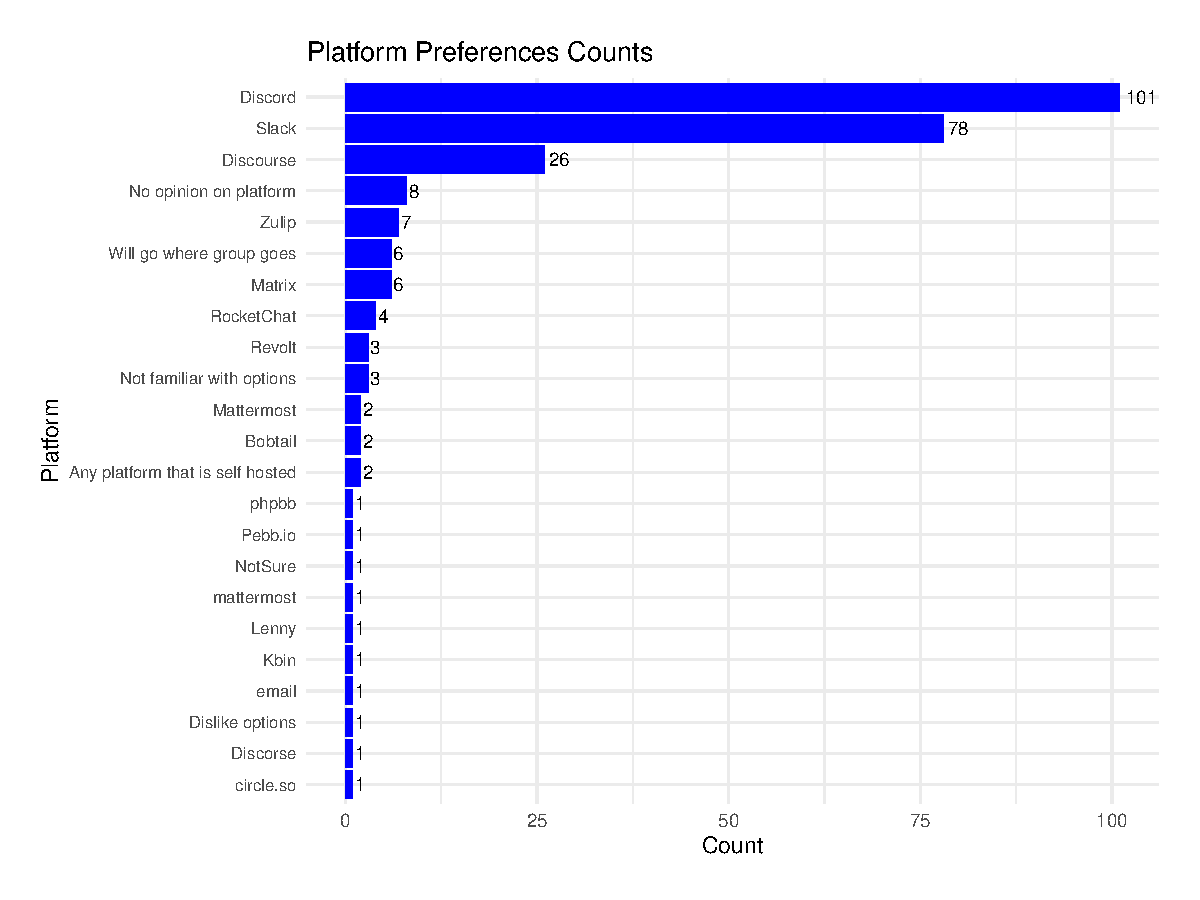
\includegraphics{XOXO_CommunitySurvey_2024_files/figure-latex/platform-barchart-1.pdf}

The favorite was Discord, followed closely by Slack and then Discourse. The question was multiple select, so folks voted for as many as they wanted and there is overlap in what people responded with.

Some folks wrote in to say that they didn't know the differences between the platforms, that they didn't have an opinion and that they would follow where the group would go.

\section{Computer vs.~Mobile}\label{computer-vs.-mobile}

Survey designers were curious to know how important mobile vs.~computer usage would be for the platform. We can see clearly from the chart that most people use both, and so functionality on both mobile and computers is important.

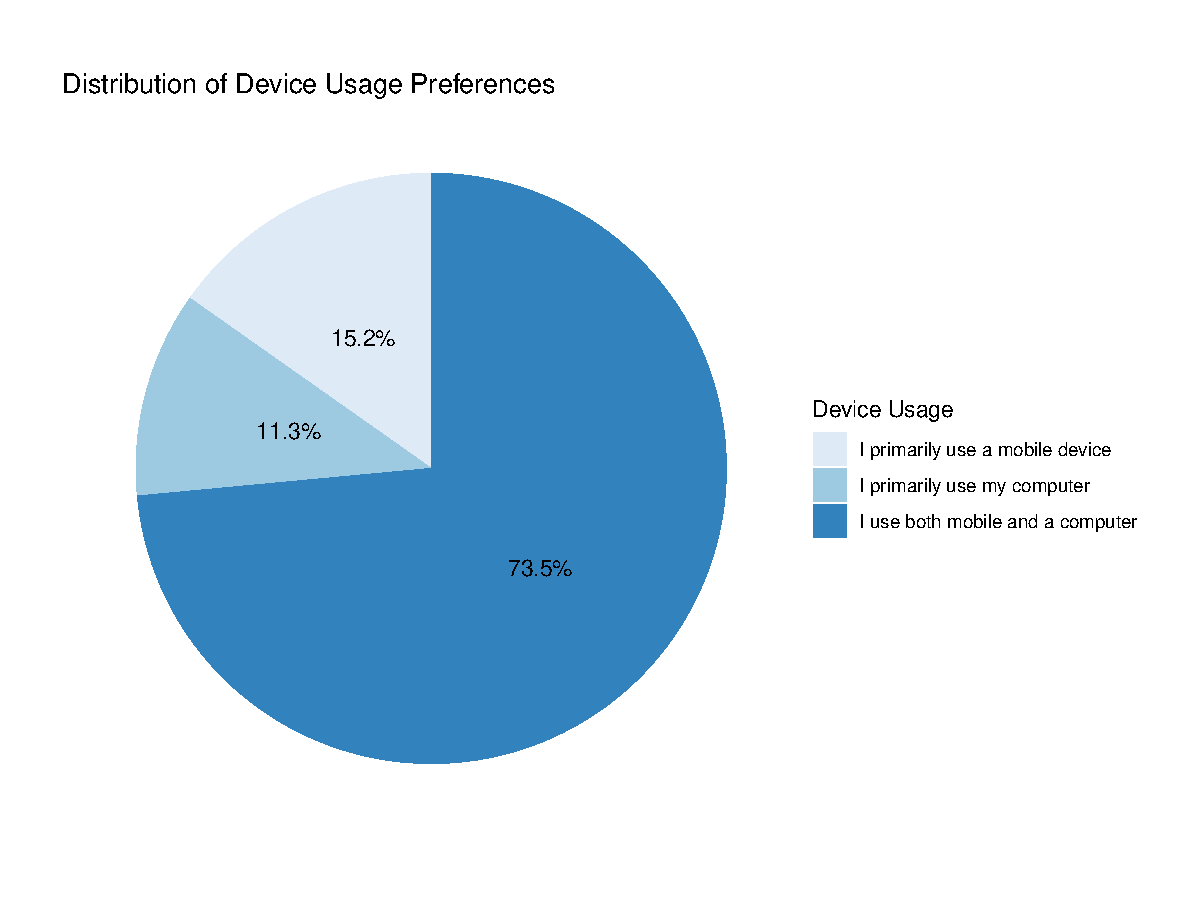
\includegraphics{XOXO_CommunitySurvey_2024_files/figure-latex/platform-piechart-1.pdf}

\chapter{Platform Opportunities}\label{platform-opportunities}

We asked people ``What opportunities (if any) do you think exist in moving to a new platform(s)?''

\section{Global Comments}\label{global-comments}

Some of the global/overall comments seem helpful to start with because there's some clarity that the community has a lot of existing capacity to create something new.

\begin{itemize}
\tightlist
\item
  We can see the whole community at a high-level and filter out what we know, after 5 years, what does and doesn't work. More importantly, we're on a deadline to gather and consolidate the collective desires in our interactivity and how our interests overlap.
\item
  There are many people in the XOXO community interested in and capable of innovating the design and maintenance of social spaces, and it's compelling to think that we could use the community tooling itself as a playground for this community, both for fun and for reinforcing the values and interests of the community. If we're careful to be inclusive (e.g.~have a baseline offering that most people can use to find others), this could take the form of an evolving set of multiple connected tools and sub-communities.
\item
  Longevity. Salesforce buying Slack curbed its innovation long-term. From experience, every SF acquisition eventually favors B2B SaaS clients so eventually it will push out communities like XOXO. I don't love Discord, but its adoption by niche active gaming communities almost guarantees future updates and support.
\item
  A lot of the talks at this year's festival acknowledged that we can have nostalgia for the early internet, but we can't go back. Moving to a new platform is part of the work of finding new paradigms (I'm sorry I said paradigm) to be creative and happy on the internet. We'll be actually doing the messy work of moving forward with our values.
\item
  ``moving away from XOXO-centric opens the door for mindful expanse of the group beyond''``I got lucky in a lottery and had money/time to spare that year''\,''
\item
  I think it also makes it more likely we'll see meaningfully active local groups which seems like a fun bonus''
\item
  ``For all the concerns I shared around losing the connection to the Andys or the physical events, having something the community feels ownership over feels arguably more values-aligned with XOXO than the existing model.
\item
  Although there are people who dislike Discord for valid reasons, I also do think it is legitimately a better tool for fostering community than Slack, and would be excited to see us adopt a tool earnestly meant for social communities instead of coopting a business tool.''
\end{itemize}

\section{Community Shifts}\label{community-shifts}

A number of the comments that we saw talked about the way that these moves could have positive impacts on the community.

\subsection{Expansion of the Community}\label{expansion-of-the-community}

The community could begin to bring more folks into it and to expand to focus on more folks.

\begin{itemize}
\tightlist
\item
  I'd love to invite trusted friends who could benefit from and add to the culture of this space.
\item
  fluidly filling a new container, adapting slack culture to a new space
\item
  Looking outside XOXO for like-minded people. It was the beacon or lighthouse that attracted us but I know there are more people that could be invited outside the physical connection of a (sadly, of course!) defunct festival in Oregon.
\item
  Oops, guess I answered this in the previous answer. TLDR: making something beyond XOXO while still staying true to its ethos. Like a vampire, I crave new blood.
\item
  growing more than one small community
\item
  ``moving away from XOXO-centric opens the door for mindful expanse of the group beyond''``I got lucky in a lottery and had money/time to spare that year''\,''
\item
  I think it also makes it more likely we'll see meaningfully active local groups which seems like a fun bonus''
\item
  It's not really platform-specific but, I like the idea that it might be possible to admit some adjacent people who weren't eligible before (e.g., XOXO attendees from before the slack existed).
\item
  Fresh starts, chance to bring in new people and spread our ethos
\item
  Being able to grow the community. I am sure there are plenty of kind, thoughtful, and creative people who would fit in.
\end{itemize}

\subsection{Evolution of the Community}\label{evolution-of-the-community}

Others also talked about the ways that the community itself could evolve and get more engaged.

\begin{itemize}
\tightlist
\item
  tighter-knit community
\item
  The potential for adding new users over time for ongoing evolution
\item
  There are many people in the XOXO community interested in and capable of innovating the design and maintenance of social spaces, and it's compelling to think that we could use the community tooling itself as a playground for this community, both for fun and for reinforcing the values and interests of the community. If we're careful to be inclusive (e.g.~have a baseline offering that most people can use to find others), this could take the form of an evolving set of multiple connected tools and sub-communities.
\item
  I'm not sure, but am happy to evolve
\item
  Gathering up a new mix of people, hopefully including others who were not previously active. Making space for the next incarnation --- more freedom and authenticity, less nostalgia and baggage.
\item
  Being able to grow the community. I am sure there are plenty of kind, thoughtful, and creative people who would fit in.
  Potentially using different technologies to facilitate different flavors of conversation.
\item
  Keeping the community going!
\item
  Self sufficiency. The Andys have created something truly wonderful and it is time for us to take on the joy/duty of caring for it.
\item
  Moving to where other communities tend to be
\end{itemize}

\subsection{Community Refresh}\label{community-refresh}

Some folks talked about wanting a refresh in the community, to redefine and to reimagine ourselves as a community.

\begin{itemize}
\tightlist
\item
  Fresh start in leadership and moderation.
\item
  I think it would be nice to start anew -- 10 years is a long time for a slack, and many channels have become quite stagnant. I'd love for a realignment of channels focused on things people are into right now.
\item
  It's a nice time to discuss likes/dislikes, implement new ideas, and refresh policies.
\item
  A fresh community start. Possibly inviting new people who share the same values and excitement, but never were able to attend or get picked for XOXO.
\item
  freedom from the planet-destroying idea that every single message ever sent MUST be archived
\item
  We get to drop some of the baggage that made the community inaccessible to newcomers. I also think we get a slight cultural reset. I've gotten a couple of passive aggressive DMs about threading --- I \emph{really} hope that behavior gets left on Slack.
\item
  Revive some of the quieter subgroups. Merge and rearrange the \#topic-list.
\item
  Fresh starts, chance to bring in new people and spread our ethos
\item
  We can redefine ourselves outside of the conference. Maybe it will give us a purpose.
\item
  potentially restructuring channels, finding new ways for channels to be visible. I really like discord's way of grouping channels
\item
  Gathering up a new mix of people, hopefully including others who were not previously active. Making space for the next incarnation --- more freedom and authenticity, less nostalgia and baggage.
\item
  might inspire people to be active again and rediscover it.
\end{itemize}

\subsection{Intentionality}\label{intentionality}

Folks talked about the intentionality of this community and how using that skill could be a helpful bonus to decide what's next.

\begin{itemize}
\tightlist
\item
  having to deliberately make new community events instead of just hoping for another XOXO conference
\item
  It's a nice time to discuss likes/dislikes, implement new ideas, and refresh policies.
\item
  There are many people in the XOXO community interested in and capable of innovating the design and maintenance of social spaces, and it's compelling to think that we could use the community tooling itself as a playground for this community, both for fun and for reinforcing the values and interests of the community. If we're careful to be inclusive (e.g.~have a baseline offering that most people can use to find others), this could take the form of an evolving set of multiple connected tools and sub-communities.
\item
  Better defining values and what we want the community to be going forward
\item
  Be more intentional in what we expect from this community.
\item
  An explicit documentation of our values
\item
  Fresh starts always have some benefit - especially if one is thoughtful about it.
\item
  Self sufficiency. The Andys have created something truly wonderful and it is time for us to take on the joy/duty of caring for it.
\item
  Intentionally strengthening the communities around channels that we realize are important to us and we'd miss.
\end{itemize}

\subsection{Opportunities from Decentralization}\label{opportunities-from-decentralization}

Some folks also specifically talked through the ways that a decentralized

\begin{itemize}
\tightlist
\item
  fluidly filling a new container, adapting slack culture to a new space
\item
  Splitting into smaller, more focused groups
\item
  Fresh starts, chance to bring in new people and spread our ethos
\item
  Segmenting user interests. Indie web already has a slack, maybe some channels would like to know about slack winding down and form their own small sub communities?
\end{itemize}

\subsection{Reorganizing}\label{reorganizing}

Some also spoke about reorganizing some of the less used slack channels

\begin{itemize}
\tightlist
\item
  Reorganizing channels
\item
  Better categorization really
\item
  Revive some of the quieter subgroups. Merge and rearrange the \#topic-list.
\item
  Segmenting user interests. Indie web already has a slack, maybe some channels would like to know about slack winding down and form their own small sub communities?
\item
  potentially restructuring channels, finding new ways for channels to be visible. I really like discord's way of grouping channels
\end{itemize}

\subsection{Moderation}\label{moderation}

There was a discussion around the needs for talking moderation, tools to use and better enable community.

\begin{itemize}
\tightlist
\item
  Spread around the responsibility for maintenance, moderation, funding
\item
  There might be a way to federate the content so it isn't one single burden to store?
\item
  Spread around the responsibility for maintenance, moderation, funding
\item
  Fresh start in leadership and moderation.
\item
  Discord is cheaper for one for all of us to maintain, but we'd have to establish a moderation team
\item
  better tools for moderation and virtual hangouts
\item
  Better moderation and better interface for writing
\item
  Discord offers better community moderation tools, bots, forum style boards, and more
\item
  I just chat, so I'm not really tuned into the mod side of things.
\end{itemize}

\subsection{Creating a Sustainable Community}\label{creating-a-sustainable-community}

Folks talked about the sustainability of the community as a part of what we're moving into and the importance of making sure that it's possible for the group to go where it makes sense to go.

\begin{itemize}
\tightlist
\item
  The Andys are/were ideal benevolent dictators, but obviously that took its toll. I'd love to maintain the pattern but make it more sustainable.
\item
  Self sufficiency. The Andys have created something truly wonderful and it is time for us to take on the joy/duty of caring for it.
\item
  Mainly avoiding getting the rug yanked out from under us at any second (eg Suddenly, A Massively Expensive Slack Plan)
\item
  Longevity. Salesforce buying Slack curbed its innovation long-term. From experience, every SF acquisition eventually favors B2B SaaS clients so eventually it will push out communities like XOXO. I don't love Discord, but its adoption by niche active gaming communities almost guarantees future updates and support.
\item
  Discord servers are easy to join once you have an account, so the community won't dwindle away
\item
  the opportunity to make an online community sustainable over time
\end{itemize}

\section{Newness}\label{newness}

Some folks talked about ways this shift could create opportunities for new ideas, new people, new events.

\subsection{New Energy}\label{new-energy}

At first we might consider the new energy that this would create

\begin{itemize}
\tightlist
\item
  I think it would be nice to start anew -- 10 years is a long time for a slack, and many channels have become quite stagnant. I'd love for a realignment of channels focused on things people are into right now.
\item
  It's a nice time to discuss likes/dislikes, implement new ideas, and refresh policies.
\item
  There are many people in the XOXO community interested in and capable of innovating the design and maintenance of social spaces, and it's compelling to think that we could use the community tooling itself as a playground for this community, both for fun and for reinforcing the values and interests of the community. If we're careful to be inclusive (e.g.~have a baseline offering that most people can use to find others), this could take the form of an evolving set of multiple connected tools and sub-communities.
\item
  Oops, guess I answered this in the previous answer. TLDR: making something beyond XOXO while still staying true to its ethos. Like a vampire, I crave new blood.
\item
  Possibly more control, ability to try and enjoy something new
\item
  Fresh starts always have some benefit - especially if one is thoughtful about it.
\end{itemize}

\subsection{New People}\label{new-people}

And many folks wanted to invite trusted people into the community and to be able to welcome them in carefully.

\begin{itemize}
\tightlist
\item
  I'd love to invite trusted friends who could benefit from and add to the culture of this space.
\item
  The potential for adding new users over time for ongoing evolution
\item
  Being able to welcome more people into the community---though that has to be done carefully as well.
\item
  A fresh community start. Possibly inviting new people who share the same values and excitement, but never were able to attend or get picked for XOXO.
\item
  Open to new members
\item
  Looking outside XOXO for like-minded people. It was the beacon or lighthouse that attracted us but I know there are more people that could be invited outside the physical connection of a (sadly, of course!) defunct festival in Oregon.
\item
  Opening to new users thoughtfully
\item
  Opening the community beyond XO attendees
\item
  Figuring out a process to invite like-minded people who haven't been to XOXO
\item
  ``moving away from XOXO-centric opens the door for mindful expanse of the group beyond''``I got lucky in a lottery and had money/time to spare that year''\,''
\item
  I think it also makes it more likely we'll see meaningfully active local groups which seems like a fun bonus''
\item
  Self hosted data, possibly opening to new people (XOXOers before 2014 aren't on the Slack, for example)
\item
  It's not really platform-specific but, I like the idea that it might be possible to admit some adjacent people who weren't eligible before (e.g., XOXO attendees from before the slack existed).
\item
  Fresh starts, chance to bring in new people and spread our ethos
\item
  Gathering up a new mix of people, hopefully including others who were not previously active. Making space for the next incarnation --- more freedom and authenticity, less nostalgia and baggage.
\item
  opportunity to build strong ways of vetting \& bringing in new members to the community
\end{itemize}

\subsection{New Resources}\label{new-resources}

Folks also wanted to make sure that the connections and resources could be central.

\begin{itemize}
\tightlist
\item
  Have a directory to the URLs of all the brilliant shared projects, resources, show and tells etc.
\item
  Other types of interaction/ collaboration?
\item
  Segmenting user interests. Indie web already has a slack, maybe some channels would like to know about slack winding down and form their own small sub communities?
\item
  New ways to interact with each other.
\end{itemize}

\subsection{New Events}\label{new-events}

A few folks talked about the possibility of events.

\begin{itemize}
\tightlist
\item
  having to deliberately make new community events instead of just hoping for another XOXO conference
\item
  New community-centric features that slack didn't offer. More regular events that are easier to organize than a large conference
\end{itemize}

\section{Specific Features}\label{specific-features}

Folks brought up the ways in which new platforms could offer new features that could enhance the community. From voice chat, to community moderation tools to more archival capabilities.

\begin{itemize}
\tightlist
\item
  Slack is a business tool by design, so some community features common on other platform are missing. (muting keywords, ignoring people, reporting folks, etc)
\item
  New community-centric features that slack didn't offer. More regular events that are easier to organize than a large conference
\item
  If Discord, there are a variety of bots/tools to help with roles/moderation/labels. Also, voice and video chatting could provide new community spaces.
\item
  Better moderation and better interface for writing
\item
  trying out new formats can be fruitful
\item
  Discord offers better community moderation tools, bots, forum style boards, and more
\item
  Private channels could have their own separate communities maybe?
\item
  Moving to discord would allow us to have streaming or voice discussions in a much more visible way than slack, otherwise I'm pretty interested in what different features other platforms offer (I just don't know enough about them to vote for them).
\item
  There might be a way to federate the content so it isn't one single burden to store?
\item
  Honestly I'm most excited about Discord because it has built in group voice chat rooms
\item
  Better options to categorize and save resources
\item
  Mainly just keeping it alive, and any potential features that might improve the experience, but I have no specifics.
\item
  Some of the new platforms are really nice and fun.
\item
  increased privacy protection, hosting our own data, having a forum space that is not real-time
\item
  Possible easier video / voice chats? Not sure if that's what people (or even I) would need, but might make it easier for groups to get together.
\item
  Better channel discoverability, avenues for intentional archival (e.g.~community cookbook)
\item
  Potentially using different technologies to facilitate different flavors of conversation.
\end{itemize}

\section{Pros to using Discord}\label{pros-to-using-discord}

Folks also talked about the benefits of using Discord.

\begin{itemize}
\tightlist
\item
  Longevity. Salesforce buying Slack curbed its innovation long-term. From experience, every SF acquisition eventually favors B2B SaaS clients so eventually it will push out communities like XOXO. I don't love Discord, but its adoption by niche active gaming communities almost guarantees future updates and support.
\item
  Discord offers better community moderation tools, bots, forum style boards, and more
\item
  Moving to discord would allow us to have streaming or voice discussions in a much more visible way than slack, otherwise I'm pretty interested in what different features other platforms offer (I just don't know enough about them to vote for them).
\item
  Discord servers are easy to join once you have an account, so the community won't dwindle away
\item
  ``For all the concerns I shared around losing the connection to the Andys or the physical events, having something the community feels ownership over feels arguably more values-aligned with XOXO than the existing model.
\item
  Although there are people who dislike Discord for valid reasons, I also do think it is legitimately a better tool for fostering community than Slack, and would be excited to see us adopt a tool earnestly meant for social communities instead of coopting a business tool.''
\item
  Honestly I'm most excited about Discord because it has built in group voice chat rooms
\item
  I use Discord more
\item
  potentially restructuring channels, finding new ways for channels to be visible. I really like discord's way of grouping channels
\item
  If Discord, there are a variety of bots/tools to help with roles/moderation/labels. Also, voice and video chatting could provide new community spaces.
\end{itemize}

\section{No/Don't Know}\label{nodont-know}

\begin{itemize}
\tightlist
\item
  Minimal if any
\item
  ¯\_(ツ)\_/¯
\item
  Stay as it is, please :)
\item
  IDK!
\item
  I just chat, so I'm not really tuned into the mod side of things.
\item
  Online tools are not my wheelhouse so I can't speak to this so much
\end{itemize}

\chapter{Platform Concerns}\label{platform-concerns}

We asked people ``What concerns (if any) do you have about moving to a new platform(s)?''

Concerns extended from responses in previous questions.

\section{Overall Concerns}\label{overall-concerns}

We had a number of overall concerns about a new platform or platforms that the group might move to.

\subsection{Folks will Disperse}\label{folks-will-disperse}

A fear we heard was that folks in the community would disperse. Folks again used language like fragmentation, splintering, fizzle out and more.

\begin{itemize}
\tightlist
\item
  strong opinions about platforms driving fragmentation
\item
  Splintering of the community, losing people
\item
  That we lose people or that communities fragment or splinter. Maybe that's ok?
\item
  It seems inevitable that some splintering will occur.
\item
  Loss of participation and splintering of interests / groups. Having yet another place to track (I belong to a lot of * slack communities and use it at work, so it's a natural part of my day. I tried with Discord, but they always fizzle * out).
\item
  My concerns about a (possible) platform migration are that 1) we fracture across multiple and not everybody makes it to a single new place, and 2) the group settles on an OSS solution that I have to jam into my life. I already have enough software to deal with in this mortal coil, I would like to avoid adding a piece of ugly, user-hostile OSS into that mess.
\item
  losing people from inertia and from the learning curve of a new technology
\item
  We seem likely to lose a lot of folks, particularly if we pick an obscure platform
\item
  we'd lose people in the transition without a path for XOXO community members to join in future
\item
  Fragmentation of the user base
\item
  community drift, or worse, schism. Or dissuaded by poor software
\end{itemize}

\subsection{Loss of Network}\label{loss-of-network}

Folks were very fearful of losing people or folks not following to the new platform. Among the ways this was phrased:

\begin{itemize}
\tightlist
\item
  I don't want to lose people (now or in the future)
\item
  General worries that people won't follow
\item
  Splintering of the community, losing people
\item
  Unavoidable, but we're going to lose a significant number of folks
\item
  If everyone will go
\item
  Losing the focus and purpose and user-base.
\item
  Loss of members
\item
  Losing lots of users
\item
  Not being able to bring many folks with it
\item
  Loss of the supportive, diverse community
\item
  Loosing stragglers
\item
  Fragmentation of the user base
\item
  Who will join the new platform?
\item
  We will lose a large number of users that are sometimes-posters
\item
  just getting everybody there
\item
  Unintentionally leaving some folks behind
\end{itemize}

Some folks talked a little more about these concerns

\begin{itemize}
\tightlist
\item
  I think moving to a new platform could have a lot of friction that causes the existing membership to shrink dramatically. I think that's especially true if the new platform is particularly complex, difficult to learn, or has limited support on people's platforms of choice.
\item
  It is probably impossible to move the near-decade of history to a new place without losing something
\item
  Learning curve and difficulty learning new interface. Loss of community as a result of friction.
\item
  It seems inevitable that some splintering will occur.
\item
  too much attrition due to learning a new platform and having to build new behaviors
\item
  That the learning curve will cause me to drop off and that the community will get a lot smaller. It's going to feel different and that scares me, though if we are able to have weekly summaries of what is being discussed, that would make everything a lot less scary and overwhelming.
\item
  losing people from inertia and from the learning curve of a new technology
\item
  We seem likely to lose a lot of folks, particularly if we pick an obscure platform
\item
  we'd lose people in the transition without a path for XOXO community members to join in future
\item
  That it would be too different and people may no longer feel comfortable as a result, and reduce/end their involvement as a result.
\item
  lose people who only occasionally check-in, hope there is a generous window or an opportunity to validate that you went to xoxo with no expiration
\end{itemize}

Some feared the loss would be driven by bad software:

\begin{itemize}
\tightlist
\item
  community drift, or worse, schism. Or dissuaded by poor software
\item
  Inevitably, not everyone will move to the same platform.
\item
  Losing a lot of people no matter where we go; having a hard time following threads in Discord
\item
  drop off of people who don't go to the new platform. Friction on the new platform that makes people not want to use it.
\item
  Losing people along the way. Adding another piece of software to my rotation.
\item
  That we would lose people in the transition, particularly if it's difficult to use. Installing yet another app on my phone.
\item
  Loss of participation and splintering of interests / groups. Having yet another place to track (I belong to a lot of slack communities and use it at work, so it's a natural part of my day. I tried with Discord, but they always fizzle out).
\end{itemize}

Some folks also remarked that they had fears, but maybe it'd be ok:

\begin{itemize}
\tightlist
\item
  Losing too many community members, but also it might be ok.
\item
  That we lose people or that communities fragment or splinter. Maybe that's ok?
\end{itemize}

\subsection{Unfamiliarity with a New Platform}\label{unfamiliarity-with-a-new-platform}

The task of a new platform being unfamiliar was a real concern for a number of folks.

\begin{itemize}
\tightlist
\item
  Onboarding/getting folks used to the platforms. Folks feeling apprehensive to move to a new platform because of effort and overwhelm. People not being aware of the new platform existing (I trust y'all to try and reach everyone to communicate the news, though!)
\item
  Myself or my peers not knowing how to use it
\item
  UI is hard for me. Discord is hard for me to keep up with - the lack of threading is really hard
\item
  Learning a new platform can be asking a lot. Slack is easy. I'm open to anything I have anxiety around navigating a new space regardless of platform
\item
  I think moving to a new platform could have a lot of friction that causes the existing membership to shrink dramatically. I think that's especially true if the new platform is particularly complex, difficult to learn, or has limited support on people's platforms of choice.
\item
  drop off of people who don't go to the new platform. Friction on the new platform that makes people not want to use it.
\item
  Discord threading is not ideal. People new to Discord may need guidance to customize it. New platforms will inevitably lose some people in the transition.
\item
  I wouldn't want the major platform decisions to alienate members of the community. I like the old nerd tilde.club-style social tech, but only a minority of our community would be willing to participate in that, and many just can't. I support the accessibility needs of the community and recognize the importance of mobile clients. As much as I would enjoy tech more open and less dependent upon capitalists, a fully hosted solution might be the only pragmatic choice that is as inclusive as we need it to be.
\item
  If it's a new app that I don't already use, I'm very unlikely to download it or use it with any regularity
\item
  It feels like Discord is the obvious choice, and maybe the right one for the bulk of the community. But I personally find Discord incredibly difficult and confusing to use, and almost certainly would drop off if that's where xoxo goes. Which, fine, my needs don't get to trump broader needs, but it makes me sad.
\item
  Most of my communities are Slack-based, so I'm going to have to get to used to something new
\item
  Learning curve and difficulty learning new interface. Loss of community as a result of friction.
\item
  The platform being clumsy and not as fun. Privacy and data ownership. Data portability.
\item
  I find Discord to be much more confusing than Slack, but would migrate to follow the community. Tbh there's a non-zero chance I would fall off after a few months. I found my way back to XOXO Slack after a few years away and was very grateful that the basic setup/layout stayed the same. I hope we don't migrate again once the new platform is found!
\item
  Losing people along the way. Adding another piece of software to my rotation.
\item
  i won't download a new app to my phone. so i am mostly concerned about moving to something that does not have a browser option
\item
  Onboarding/getting folks used to the platforms. Folks feeling apprehensive to move to a new platform because of effort and overwhelm. People not being aware of the new platform existing (I trust y'all to try and reach everyone to communicate the news, though!)
\item
  That the learning curve will cause me to drop off and that the community will get a lot smaller. It's going to feel different and that scares me, though if we are able to have weekly summaries of what is being discussed, that would make everything a lot less scary and overwhelming.
\item
  That we would lose people in the transition, particularly if it's difficult to use. Installing yet another app on my phone.
\item
  the community is made of a lot of technically competent people, and I worry that our new technology will be too cumbersome to be a part of our everyday life. With the fracturing of social media there's already too many things to check.
\item
  Loss of participation and splintering of interests / groups. Having yet another place to track (I belong to a lot of slack communities and use it at work, so it's a natural part of my day. I tried with Discord, but they always fizzle out).
\item
  My concerns about a (possible) platform migration are that 1) we fracture across multiple and not everybody makes it to a single new place, and 2) the group settles on an OSS solution that I have to jam into my life. I already have enough software to deal with in this mortal coil, I would like to avoid adding a piece of ugly, user-hostile OSS into that mess.
\item
  I'm going to have to download yet another app.
\item
  It won't be as easy to access or read on mobile. That I will lose access because I don't post.
\item
  losing people from inertia and from the learning curve of a new technology
\item
  We seem likely to lose a lot of folks, particularly if we pick an obscure platform
\item
  Nothing specific other than the mental overhead
\item
  Honestly if it's significantly less convenient (I use slack for work) then I don't think I'll read or contribute to it as much
\item
  ADHD will be too challenging
\item
  Learning a new platform might cause friction that drives pepole away.
\item
  Friction in moving to new platform; degraded experience on either desktop or mobile
\end{itemize}

\subsection{Loss of Resources}\label{loss-of-resources-1}

Some folks addressed their concerns about losing resources we have.

\begin{itemize}
\tightlist
\item
  Losing core functionality (like threading) that has helped structure the space. Biggest concern would be whether we can keep the vibe alive. Good, kind-hearted humans helping and supporting each other, and sharing information that is vetted and trustworthy. I also worry about moving to a platform that's going to shut down sooner rather than later.
\item
  feeling like its the same community even if its in a new space (e.g.~is this a place where I'd complain about ants to? celebrate wins with? post cat pics in?)
\item
  Loss of access to old posts, media, etc.
\end{itemize}

\subsection{Governance and Moderation}\label{governance-and-moderation}

Several folks shared their concerns around governance.

\begin{itemize}
\tightlist
\item
  What is the governance?
\item
  being too insular and rigid, allowing the community to evolve
\item
  The loudest voices over powering the majority, the community petering out, not deciding where to move and splintering
\end{itemize}

Specifically folks were concerned about the workload for volunteers and making sure that the volunteers don't burn out and that the vibes stay

\begin{itemize}
\tightlist
\item
  Making sure moderation and vibes stay
\item
  Not everyone migrating, lack of moderation possibly, not being default might mean people will be less active
\item
  The organisation and moderation of the slack was impeccable, it'll take a while to migrate that to a new platform, especially without the two Andy's as guide posts
\item
  Moderation, keeping to the XOXO Slack code of conduct
\item
  Lack of moderation tools, loss of asynchronous discussion
\item
  Choosing one that doesn't provide the admin/moderation tools we need to run it the best way for our community
\item
  The moderation
\item
  Moderation. XOXO has always been The Andy's Place, so playing by their rules and the community norms that emerged from that starting point made it seem like things were already sorted out by the time I joined in 2017. But who makes those decisions, and how, once we are in The Next Place will be curious.
\item
  The level of (likely invisible) labor required to actively moderate the community and how to make it sustainable
\item
  we need strong, trusted moderators
\item
  organizer burnout; admin tax (if maintaining the software); paid moderation
\item
  Impact on facilitators/moderators
\item
  Maintaining a community is hard, and we'll be losing the physical space binding XOXO together. I'm particular concerned about volunteer moderator burnout.
\item
  the community is made of a lot of technically competent people, and I worry that our new technology will be too cumbersome to be a part of our everyday life. With the fracturing of social media there's already too many things to check.
\end{itemize}

\subsection{Corporations and Money}\label{corporations-and-money}

Folks had concerns about corporate platforms and what those platforms might mean for the members of the community.

\begin{itemize}
\tightlist
\item
  Locking into another potentially unstable, objectionable corporate platform
\item
  Moving to another corporate platform like Discord of course has its risks. Their monitezation hooks are already obnoxious, but it still feels like the best fit for this community. I also worry about the opposite problem of persuing an open source/self hosted platform that is frustrating/alienating to use for most people. Doesn't feel like there are any perfect soluations out there, so we just have to make the best decision we can.
\item
  Longevity. Newer platforms sound promising but we all know how easily things can be shut down without notice
\item
  I wouldn't want the major platform decisions to alienate members of the community. I like the old nerd tilde.club-style social tech, but only a minority of our community would be willing to participate in that, and many just can't. I support the accessibility needs of the community and recognize the importance of mobile clients. As much as I would enjoy tech more open and less dependent upon capitalists, a fully hosted solution might be the only pragmatic choice that is as inclusive as we need it to be.
\item
  Opening to new users thoughtlessly, vulnerability to changing priorities from platform owners
\item
  Losing core functionality (like threading) that has helped structure the space. Biggest concern would be whether we can keep the vibe alive. Good, kind-hearted humans helping and supporting each other, and sharing information that is vetted and trustworthy. I also worry about moving to a platform that's going to shut down sooner rather than later.
\item
  Discord and corporate platforms will enshittify
\end{itemize}

Some also talked about issues around money and the costs

\begin{itemize}
\tightlist
\item
  Potential costs (and entities formed to cover those costs), platform rug-pulls.
\item
  I am deeply distrustful of commercial platforms. I have seen their attempts to monetize destroy communities. I have some concern that a platform change could lead to some culture change.
\end{itemize}

\subsection{Loss of XOXO Spirit}\label{loss-of-xoxo-spirit}

Folks were concerned about losing the special something that comes from the XOXO community.

\begin{itemize}
\tightlist
\item
  I wouldn't want the major platform decisions to alienate members of the community. I like the old nerd tilde.club-style social tech, but only a minority of our community would be willing to participate in that, and many just can't. I support the accessibility needs of the community and recognize the importance of mobile clients. As much as I would enjoy tech more open and less dependent upon capitalists, a fully hosted solution might be the only pragmatic choice that is as inclusive as we need it to be.
\item
  Loss of the supportive, diverse community
\item
  Losing the vibe? The Andys? I hope they join the new platform, too.
\item
  Having to rebuild a culture around new ways of doing things
\item
  It is probably impossible to move the near-decade of history to a new place without losing something
\item
  Making sure moderation and vibes stay
\item
  Losing all of the emojis.
\item
  I am deeply distrustful of commercial platforms. I have seen their attempts to monetize destroy communities. I have some concern that a platform change could lead to some culture change.
\item
  Choosing one that doesn't provide the admin/moderation tools we need to run it the best way for our community
\item
  too much attrition due to learning a new platform and having to build new behaviors
\item
  Losing core functionality (like threading) that has helped structure the space. Biggest concern would be whether we can keep the vibe alive. Good, kind-hearted humans helping and supporting each other, and sharing information that is vetted and trustworthy. I also worry about moving to a platform that's going to shut down sooner rather than later.
\item
  feeling like its the same community even if its in a new space (e.g.~is this a place where I'd complain about ants to? celebrate wins with? post cat pics in?)
\item
  That it would be too different and people may no longer feel comfortable as a result, and reduce/end their involvement as a result.
\end{itemize}

\subsection{Fears Around Newcomers}\label{fears-around-newcomers}

Some folks shared the challenges that would be associated with bringing new folks into the community.

\begin{itemize}
\tightlist
\item
  Opening to new users thoughtlessly, vulnerability to changing priorities from platform owners
\item
  the balance between stagnation and leaving the door open to assholes.
\item
  Maintaining the community while continuing to grow in a considered way.
\item
  Privacy and safety. Also, do we limit membership to folks already in the Slack? (I personally prefer this)
\end{itemize}

\section{Platform Functions}\label{platform-functions}

\subsection{Threading}\label{threading}

The function of threading in the platform emerged as a really key component of what the community needs.

\begin{itemize}
\tightlist
\item
  UI is hard for me. Discord is hard for me to keep up with - the lack of threading is really hard
\item
  Losing a lot of people no matter where we go; having a hard time following threads in Discord
\item
  Discord threading is not ideal. People new to Discord may need guidance to customize it. New platforms will inevitably lose some people in the transition.
\item
  Threading is so important
\item
  Having threads and a good search
\item
  I really like the interest-specific channels and the threads, so people can skim or go in depth
\item
  Lack of moderation tools, loss of asynchronous discussion
\item
  Losing core functionality (like threading) that has helped structure the space. Biggest concern would be whether we can keep the vibe alive. Good, kind-hearted humans helping and supporting each other, and sharing information that is vetted and trustworthy. I also worry about moving to a platform that's going to shut down sooner rather than later.
\end{itemize}

\subsection{Privacy}\label{privacy-1}

\begin{itemize}
\tightlist
\item
  ``the medium is the message'' that a different format will change the vibe significantly. Privacy, would want a non-public space (ie not twitter)
\item
  Privacy balanced with re-connecting with my Slack friends. I remember real names more than anonymous usernames. But like others, I have several usernames on other platforms: public, private, and professional. I'd like to avoid managing throwaway accounts in order to avoid doxxing.
\item
  The platform being clumsy and not as fun. Privacy and data ownership. Data portability.
\item
  Privacy and safety. Also, do we limit membership to folks already in the Slack? (I personally prefer this)
\end{itemize}

\subsection{Additional Platform Functions}\label{additional-platform-functions}

\begin{itemize}
\tightlist
\item
  It's nice to be able to see an account to a real person (like even if they use an alias/not their given name, the alias is consistent IRL/online). One issue I've had in other big Discords is someone will have a big or personal ask (ex: looking for roommates or even meeting up at an event), but ALL of their personally identifiable information is hidden and I have no idea who this anonymous asker is, as much as I would like to help or connect. Also I really hate Discord threading.
\item
  Having threads and a good search
\end{itemize}

\section{Platform Specific Discussions}\label{platform-specific-discussions}

Folks had opinions about Discord both for and against.

\subsection{Discord Pros}\label{discord-pros}

\begin{itemize}
\tightlist
\item
  Please let's just move to Discord and copy over the channels exactly. Let's keep this simple.
\item
  I really don't want us to try and spin up our own bespoke solution - having been part of many communities that tried to do that, the maintainer burden is very high and retention starts to drop fast. Let's stick with a solution that's built and has a dedicated (paid ) team behind it, like Discord or Slack.
\end{itemize}

\subsection{Discord Downsides}\label{discord-downsides}

\begin{itemize}
\tightlist
\item
  UI is hard for me. Discord is hard for me to keep up with - the lack of threading is really hard
\item
  Discord and Zulip are both an absolute nightmare from a UI \& UX perspective. You can't really leave channels in Discord.
\item
  Losing a lot of people no matter where we go; having a hard time following threads in Discord
\item
  Discord threading is not ideal. People new to Discord may need guidance to customize it. New platforms will inevitably lose some people in the transition.
\item
  I really hate discord
\item
  Discord seems harder to understand and use than Slack.
\item
  It feels like Discord is the obvious choice, and maybe the right one for the bulk of the community. But I personally find Discord incredibly difficult and confusing to use, and almost certainly would drop off if that's where xoxo goes. Which, fine, my needs don't get to trump broader needs, but it makes me sad.
\item
  Discord
\item
  I find Discord to be much more confusing than Slack, but would migrate to follow the community. Tbh there's a non-zero chance I would fall off after a few months. I found my way back to XOXO Slack after a few years away and was very grateful that the basic setup/layout stayed the same. I hope we don't migrate again once the new platform is found!
\item
  I hate Discord so much and find it unusable.
\item
  Loss of participation and splintering of interests / groups. Having yet another place to track (I belong to a lot of slack communities and use it at work, so it's a natural part of my day. I tried with Discord, but they always fizzle out).
\item
  Discord and corporate platforms will enshittify
\end{itemize}

\subsection{Slack Pros}\label{slack-pros}

Folks shared their pros for using Slack in the future.

\begin{itemize}
\tightlist
\item
  Learning a new platform can be asking a lot. Slack is easy. I'm open to anything I have anxiety around navigating a new space regardless of platform
\item
  I'm used to Slack, for all its problems \ldots{} I'm worried we will overestimate our community's desire to run/manage something bespoke (I think we should use a hosted service for sure)
\item
  I really don't want us to try and spin up our own bespoke solution - having been part of many communities that tried to do that, the maintainer burden is very high and retention starts to drop fast. Let's stick with a solution that's built and has a dedicated (paid ) team behind it, like Discord or Slack.
\item
  I find Discord to be much more confusing than Slack, but would migrate to follow the community. Tbh there's a non-zero chance I would fall off after a few months. I found my way back to XOXO Slack after a few years away and was very grateful that the basic setup/layout stayed the same. I hope we don't migrate again once the new platform is found!
\item
  Loss of participation and splintering of interests / groups. Having yet another place to track (I belong to a lot of slack communities and use it at work, so it's a natural part of my day. I tried with Discord, but they always fizzle out).
\item
  Honestly if it's significantly less convenient (I use slack for work) then I don't think I'll read or contribute to it as much
\end{itemize}

\subsection{OSS Downsides}\label{oss-downsides}

Folks talked about the downsides for doing an open source software (OSS) package

\begin{itemize}
\tightlist
\item
  Moving to another corporate platform like Discord of course has its risks. Their monitezation hooks are already obnoxious, but it still feels like the best fit for this community. I also worry about the opposite problem of persuing an open source/self hosted platform that is frustrating/alienating to use for most people. Doesn't feel like there are any perfect soluations out there, so we just have to make the best decision we can.
\item
  I'm used to Slack, for all its problems \ldots{} I'm worried we will overestimate our community's desire to run/manage something bespoke (I think we should use a hosted service for sure)
\item
  I really don't want us to try and spin up our own bespoke solution - having been part of many communities that tried to do that, the maintainer burden is very high and retention starts to drop fast. Let's stick with a solution that's built and has a dedicated (paid ) team behind it, like Discord or Slack.
\item
  the community is made of a lot of technically competent people, and I worry that our new technology will be too cumbersome to be a part of our everyday life. With the fracturing of social media there's already too many things to check.
\item
  My concerns about a (possible) platform migration are that 1) we fracture across multiple and not everybody makes it to a single new place, and 2) the group settles on an OSS solution that I have to jam into my life. I already have enough software to deal with in this mortal coil, I would like to avoid adding a piece of ugly, user-hostile OSS into that mess.
\item
  We seem likely to lose a lot of folks, particularly if we pick an obscure platform
\item
  community drift, or worse, schism. Or dissuaded by poor software
\end{itemize}

\chapter{Name}\label{name}

We asked ``What do you think the new community(ies) should be named?'' and received open responses (e.g.~there were no ideas listed for folks to choose between).

\section{Top Contenders}\label{top-contenders}

I've listed out any name that was listed on with more than two votes (including all variations) and the approximate number of votes.

\begin{itemize}
\tightlist
\item
  And, And/\&\& (8)
\item
  Enthusiasm Collective (8)
\item
  Good Internet (7)
\item
  Lowered Expectations/LoX/LOX/LowEx (5)
\item
  YNYN (2)
\item
  TKTK (2)
\item
  Good Together (2)
\end{itemize}

\subsection{Other thoughts}\label{other-thoughts}

\begin{itemize}
\tightlist
\item
  JabbawockeeBook
\item
  YOYO
\item
  The Imposters
\item
  Someplace
\item
  Elsewhere
\item
  Good Together
\item
  NeD
\item
  YOYO
\item
  TskTsk
\item
  Dandelion
\item
  With Love
\item
  and/or
\item
  ZIZI
\item
  Mutiny
\item
  Delicious Burger
\item
  Restart to update
\item
  Indie Internet Appreciation Society
\item
  Amalgamated Enthusiasm
\item
  Death Form for Cutie
\item
  Life Raft for Cutie
\item
  The Grove (or something nature/wilderness based)
\item
  Kinfolx
\item
  Murmur
\item
  A Very Low Number of Dingalings
\item
  Amalgamated Enthusiasm
\item
  Patchwork
\end{itemize}

\subsection{Inside Jokes}\label{inside-jokes}

Folks had thoughts about the name being an inside joke. While most didn't want the inside joke to be too involved, there were some that thought it would be good for it to refer back to jokes and conversations in the community.

\begin{itemize}
\tightlist
\item
  Something that's not an in-joke from the in-person stuff or would be off putting to future potential new people
\item
  YOYO. Don't really care. But I think a connection to the festival or shared values is important. Lowered Expectations and The Imposters are also good choices: festival-specific inside jokes, but also close to the values and personalities of attendees. Yo-yo works as a name since most of us are bouncing up and down between pride and insecurity.
\item
  Personally I would avoid deep in-jokes from particular years of the festival
\item
  No preference. But maybe avoid anything that's too deep of an inside joke.
\item
  I just don't want it to be an inside joke. Like the death cab or 21st September thing, neither of those resonate with me and I think they're pretty played out. Whatever it's called, it should stand on its own.
\end{itemize}

\subsection{Additional Comments}\label{additional-comments-1}

\begin{itemize}
\tightlist
\item
  please nothing with \& in it, otherwise very open
\item
  I liked Dandelion from that one thread of names.I think \&\& is fun, but also maybe annoying to refer to? Then again we've been saying X-O-X-O for a decade haha
\item
  Something that speaks to the core values of the group while being as inclusive as possible (eg no inside jokes).
\item
  Maybe a name that can evolve as the community changes.
\item
  YOYO. Don't really care. But I think a connection to the festival or shared values is important. Lowered Expectations and The Imposters are also good choices: festival-specific inside jokes, but also close to the values and personalities of attendees. Yo-yo works as a name since most of us are bouncing up and down between pride and insecurity.
\item
  Pool some money together and buy Twitter brand
\end{itemize}

\subsection{Don't Care}\label{dont-care}

Many folks did not care, didn't know or expressed a desire to use whatever the community decided.

\begin{itemize}
\tightlist
\item
  I'm open to anything
\item
  Not that important to me, tbh.
\item
  I have no strong opinion
\item
  I'll use it no matter what it's called.
\item
  Ooh I have been trying to think of a good name and cannot. I'll leave it to the more creative folks of our group lol
\item
  No good ideas here 😅
\item
  I don't have a strong preference so far. There have been a lot of clever suggestions and, I am down for whatever resonates with the most people. A rose by any other name \ldots{}
\item
  Oh gosh honestly I don't know!
\item
  I don't have a strong opinion here. I don't feel a strong need to reference the old community or conference or Andys in the name.
\item
  No preference
\item
  I'm ambivalent, or without much concern or preference for naming.
\item
  I have no idea, I accidentally named a mascot Darryl Scroggins because I hate naming things so I try to suggest bad names so people stop asking me
\item
  I really don't have an opinion here.
\item
  No idea! Naming stuff is hard
\item
  defer to the thread on slack
\end{itemize}

\subsection{Variations on XOXO:}\label{variations-on-xoxo}

The following names are likely to not be a good fit after the Andys requested we not use XOXO in the next name.

\begin{itemize}
\tightlist
\item
  The XOXO Netflix Film Community
\item
  XOXO Alum (tie)
\item
  exoh
\item
  exes
\item
  oxox? I am bad at naming things.
\item
  XOXO alumni
\item
  OXOX? Oxenfree?
\item
  Xoxo community!
\item
  OXOX
\item
  something XOXO
\item
  XOXII
\item
  Xoxo Alumni
\item
  ExOXO
\item
  OX
\item
  XO2O
\end{itemize}

\chapter{Thank You to The Andys}\label{thank-you-to-the-andys}

In the survey we offered up a chance for folks to express their gratitude. And this community took their gratitude seriously.

Buckle up folks and bring out those kleenex. Here's our community note of gratitude to you both.

Dear Andys,

You're the best, we think the world of you. You made a community, one that was kind and that helped us remember the good internet. We saw how hard you worked. You changed lives and you should be proud of what you've done. We are so grateful and we the community will take it from here. Thank you.

Love, the XOXO community

\section{You're the Best}\label{youre-the-best}

\begin{itemize}
\tightlist
\item
  the best Andy's ever.
\item
  y'all are literally THE BEST. please be proud of what you've done! I know as a creator you always compare what exists in the world with the perfect thing you imagined in your head but what you made was and is AMAZING. You did great!!
\item
  XOXO is (was?) my favorite thing. Not my favorite conference, not my favorite Slack instance. My favorite thing, period.
\item
  There are no words. What the Andys created was pure magic and will never be duplicated. Thank you for the love, laughs and tears. You are the best!
\item
  You're the best. Thank you for everything.
\end{itemize}

\section{We Think the World of You}\label{we-think-the-world-of-you}

\begin{itemize}
\tightlist
\item
  Andys, for everything wonderful about what you've made, I hope you also know that it's okay to walk away. We'll miss it, but you've already done the work and we can take it from here. It's okay for beautiful things to end, and to create space for new things to grow.''
\item
  Thank you so much Andy and Andy. The XOXO Slack Community is very special.
\item
  Thank you to the Andys and Rachel for all their consideration and mindfulness. I feel like this community has welcomed me, educated me, and included me in ways no other social community has before. It's so beautiful and I hope you never forget all you've given and what you've grown with us. Big thank you.
\item
  Andys, whether you knew it or not, you've been amazing mentors for me. So often, social (and business) spaces have been so inhuman and inhumane, and you made XOXO Slack welcoming, human, and just plain nice. Seeing it actually done for real is a huge accomplishment and an inspiration to me and others. I am so grateful. Thank you.
\item
  No small part of the magic of the XOXO community has been due to your thoughtful and careful curation. Thank you!
\item
  You two absolute mensches have poured your love into our community, have helped \emph{make} us a community and not just a herd of somewhat feral cats. You've made thoughtful choices, over and over, curating as caretaking, looking after your creation even at real cost. You are personally responsible for more \#good-internet than you can ever know. Your legacy will last as long as humans know the internet existed. Thank you for gathering up all the folks from my home planet; it was lonely before we had each other.
\item
  You guys already know I love you because I text you all the time so\ldots{} yea
\item
  ``They must already know the massive impact they've had on this community, and the internet at large. xoxo is a legendary event, and its impact will be long-reaching. They brought people together, and helped those people share ideas. What a wonderful thing to spend the rest of your life knowing that you did.
\item
  Andy Andy Andy Andy
\end{itemize}

\section{You Made a Community}\label{you-made-a-community}

\begin{itemize}
\tightlist
\item
  you made an amazing community, thank you.
\item
  This community is hands down the best thing about XOXO. I'm glad that the festival and conference was the catalyst for it.
\item
  It's rare to create such a wonderful community. I'm deeply appreciative of all the work you and all the volunteers have put into making XOXO
\item
  OMG Thank you for creating something so incredible, and so meaningful to people! Happy retirement!
\item
  XOXO has filled a spot in my heart that I didn't even know I needed. I feel so lucky to be apart of this in such a minor way. Thank you for bringing such a unique group of people together and giving them a space to share their really cool brains.
\item
  ``Communities are as much expressions of their leaders and maintainers as they are products of their members. The Andys have used their talents and experience to give us a place to be that is unlike any other online, and I am most grateful
\item
  There is grace is knowing that all things end, and recognizing the responsibility to end things well. Thank you for throwing one last party, and for ushering the XOXO Slack community towards its next evolution.''
\item
  Thank you for being brave enough, and hard working enough to build such an incredible community and experience.
\item
  Most important community in my life, my gratitude is immeasurable
\item
  This is such a special, strong, and amazing community. I really do not know how I would have gotten through having-a-baby-during-COVID without it.
\item
  I have tons of respect for how you've built up this community! I'm sad to see it end, but I think it was 100\% the correct decision. I look forward to learning about what you do next.
\item
  Thank you for all that you have done with a big nod for allowing one last gathering so members could get a sense of closure. Also, thnx for allowing the community three months to wind down and still leave what was hear archived so people can find things in the future, Very well done gentlemen.
\item
  Thanks. Believe it or not, this community has replaced MetaFilter for me, which was my previous ride-or-die. Knowing what I do about communities like this, I honestly can't believe you've been able to foster such a great place for this long. It's very smart to make this transition when things are on an upswing.
\end{itemize}

\section{A Community that was Kind}\label{a-community-that-was-kind}

\begin{itemize}
\tightlist
\item
  This has been the best-run, most useful and least-asshole-ish virtual community at scale that I've been a part of, honestly. Even just as a Portland resource for vendors, etc, it's amazing. Thank you for manifesting your kindness and thoughtfulness into this living artifact.
\item
  Thank you for creating one of the most considerate, welcoming, and respectful communities I've ever had a chance to be a part of. The festival is always great fun, but the community has been an invaluable part of my life for the past 8 years. Given how bleak those of those years have been, I'm really not sure how I'd have got through them without the constant support, company, and mutual commiseration of the XOXO community.
\item
  I am incredibly impressed by the level of kindness and goodwill that is displayed not just in the community but in your approach to building and maintaining it. I aspire to fostering similar community where I am called to do so. Thank you for putting so much of yourselves into this for so long even when I am sure it was very hard.
\item
  This community has been a real comfort to me as I navigate life. I don't know of another place where there are so many smart, lovely and supportive folks in one place.
\item
  Truly unique and powerful experiences, ripples of creativity and human connection that will continue for years and years to come. With all the kids at the last one\ldots for generations even!
\end{itemize}

\section{You Helped us Remember the Good Internet}\label{you-helped-us-remember-the-good-internet}

\begin{itemize}
\tightlist
\item
  Andys, you did something I never thought I'd ever see in the world. You created space for an increasingly diverse and varied gathering of people to get deeply into their feelings, from anger and sorrow through excitement and joy, all in the name of celebrating weird and neat things made possible by the internet and technology. What an absolutely incredible treasure this has been. Thank you.
\item
  XOXO is a remarkable, unique, and pretty much unchallenged take at creating a real-world representation of the hope and power of the connected world through technology, without forgetting that there are people around every corner, decision, design, platform, and ``product''. I will miss it but also take the experience in person and online with me with every one of my endeavors and experiences. It is an unforgettable force and experience and will difficult to move forward without remembering it, being influenced by it, or flat-out trying to steal (ok, maybe ``share'' is better) it's pure energy and power .
\item
  Thank you for keeping the spirit of the Good Internet alive, we hope to continue it
\item
  In a particular part of my life, I can only point to one other thing that has meant so much to me and that is the Internet, or maybe more specifically the web, itself. XOXO is the best of the Internet in human form. It embodies the wholesome goodness that is the Internet. When I think about it, I literally get choked up and think to myself, `how is it possible this existed and how lucky am I to have been a small part of it a few times.' I really wish I could find the words to express what it means to me. And I am just ONE of the lucky people that got to experience it. How lovely. How profound.
\end{itemize}

\section{We Saw How Hard You Worked}\label{we-saw-how-hard-you-worked}

\begin{itemize}
\tightlist
\item
  Your dedication to keeping this weird thing alive is truly inspiring. I cannot imagine the amount of effort and time it's taken to moderate this, and create such a positive structure. I guess all I can really say is: well fucking done.
\item
  Your emotional labor was not in vain and did not go unseen.
\item
  It's a lot of work to curate people and ideas, especially in a way that is inclusive, yet expansive. Thank you, Andy's, for creating the space for us to connect, learn, experience joy, share angst, collaborate on ideas and tools to express the best part of ourselves.
\item
  Thank you for all of the hard work and thought you put into the slack community over the years to make it such a welcoming and empathetic space that I now feel devastated to lose!
\item
  Community moderation is hard but you make it look easy
\end{itemize}

\section{You Changed Lives}\label{you-changed-lives}

\begin{itemize}
\tightlist
\item
  Thank you from the bottom of my heart. XOXO changed my life and I appreciate the phenomenal effort you have put into creating a space where people feel safe to be their true selves. You have done something truly amazing and connected hundreds of people in a way that I don't think any other community I encounter will ever compare.
\item
  In terms of life's work, this is pretty excellent.
\item
  Thank you for creating a wonderful community! The XOXO conference has been life-changing. I'm so sad that it's the last IRL time, but I'm glad I got to attend multiple times.
\item
  Y'all have changed my life, multiple times, since my first XOXO in 2015. I literally wouldn't be here without you and what you've helped create. I will never be able to repay that, but I try every day. Thank you seems insufficient, but it's a start: thank you.
\item
  I firmly believe that the XOXO community saved lives during the Trump administration and the pandemic, and I am thankful for that. I came for the talks and found a community.
\item
  They created a lifeline and one of the few places where I feel hopeful, understood, and welcome. They also have modeled how to be a better person.
\item
  Thank you. I'm not the same person I was in 2012 when I attended my first XOXO and as the community grew and changed, so did I. Thank you for starting something special and caring enough to continue it despite challenges. When I reflect on XOXO, it's one of the most life changing things I could've encountered and feel lucky and fortunate for the friendships I've made and the lessons I've learned over the past 12 (wow!) years
\end{itemize}

\section{You Should be Proud}\label{you-should-be-proud}

\begin{itemize}
\tightlist
\item
  I think y'all should be really proud of what you built! It was an amazing experience for so many people and I'm grateful I got to be part of it.
\item
  You should be so proud
\item
  You should be very proud. And yet, in the many years I've known you, you remain humble and practically defiant of any ego. You not only built a festival and an event that remains my standard of excellence, but you also fostered a decade-long community with shared values and creative curiosity across a variety of mediums and niche interests. Your leadership is aspirational: you come to the table with big ideas but also practical next steps, you proactively plan for inclusivity instead of the bare minimum of reactionary accessibility, and you empower self-organization in the community and amongst support staff while balancing appropriate management with genuine encouragement. The XOXO community has been indescribably my closest network---inspirational, supportive, and empathetic. While the final festival and archiving of the Slack workspace is bittersweet, it's also a cathartic transition I needed post-2020.
\end{itemize}

\section{We are So Grateful}\label{we-are-so-grateful}

\begin{itemize}
\tightlist
\item
  i'm so grateful for the work y'all put in on this whole thing\textasciitilde{}
\item
  Thank you for the opportunity to be in Portland in 2018 gratis. It was a meaningful experience that continues to impact my life positively.
\item
  So much gratitude and appreciation. thank you again.
\item
  I am grateful- so grateful
\item
  I feel very lucky to have been able to be a part of such a wonderful community and I am deeply, deeply grateful that it existed to begin with.
\item
  Thank you. With every ounce of love that I can muster from every corner of my heart, thank you.
\item
  You have enough folks telling you, you've created something special and that it'll be missed. I hope you get to see the 1000s of flowers bloom that you seeded here, thank you for everything \textless3
\end{itemize}

\section{We Got It From Here}\label{we-got-it-from-here}

\begin{itemize}
\tightlist
\item
  Gentlemen, thank you, and please take a break, toast each other with a beverage, and know you've built a great place. To quote an album title, We got it from here, thank you for your service.
\item
  Enjoy your rest, we've got it from here!
\item
  You created this community and you will always be a part of it, but you don't have to worry. We've got it. Time for us to leave the nest.
\item
  Thank you. You couldn't have known what we would become and thank you for supporting this cultural experiment. We're ready for what's next.
\end{itemize}

\section{All The Thank You's}\label{all-the-thank-yous}

Thank you, thank you, thank you! I hope I get to see what you each do next.
Thank you!
Thank you
Thank you so much for all you've done in creating this wonderfully kind little slice of the internet.
Thank you for years of XOXO and curating this community
THANK YOUUUUUUUUUU
Thank you, for everything!
thank you for 10+ years of what came to be my favorite online community.
Thank you.
thank you, you have changed my life for the better!
Thank you.
Thank you.
Thank you. Really--- thank you.
Thank you. A big heartfelt thank you.
Thanks a lot, guys, it's been such a fun ride
A million, million thank yous!
Thanks guys. You made the thing, and it mattered to people.
Thank you! You made something good in the world.
Thank you!!
Thank you!
Thank You so very very very much
Thank you for this gift to the world.
Wow!
Thank you, you've done a good thing here.
Thank you for making such a beautiful community of brilliant minds.
Thank you!!
Words can't do it justice, but a very sincere thank you.
Thank you so much--I cannot express how much you have changed my life!
There's a lot I could say, but all of it is: ``thank you''
Thank you, thank you, thank you!
Thank you for giving so much of yourselves.
Thank you Andys! This is a really really special community. I feel so fortunate to get to be a part of it.
Thank you. You raised my expectations
Thank you!!!
Thank you for creating a corner of the internet and real life that didn't succumb to enshittification.
Thank you for everything. Thank you very, very, very much.
Thank you.
good job!
Just immense thanks and gratitude.
thank you for this incredible community
Thank you for bringing such wonderful people together.
\textless3

\chapter{Appendix - Survey Questions}\label{appendix---survey-questions}

\begin{itemize}
\tightlist
\item
  If you were to briefly summarize the core values of the XOXO Slack community as it exists now, what would they be?
\item
  What do you appreciate about the XOXO Slack community?
\item
  What (if any) concerns do you have as you the XOXO Slack winds down?
\item
  Which of the following platforms would you most like to see the XOXO community migrate to?
\item
  Click which of the following is true for you as you currently access the XOXO Slack:
\item
  What opportunities (if any) do you think exist in moving to a new platform(s)?
\item
  What concerns (if any) do you have about moving to a new platform(s)?
\item
  What do you think the new community(ies) should be named?
\item
  What would you like to share publicly about how the XOXO Slack has impacted your life?
\item
  If you'd like to say anything to the Andys about what they created, feel free to do so here.
\item
  Anything else you'd like to share?
\end{itemize}

  \bibliography{book.bib,packages.bib}

\end{document}
